% Options for packages loaded elsewhere
\PassOptionsToPackage{unicode}{hyperref}
\PassOptionsToPackage{hyphens}{url}
\PassOptionsToPackage{dvipsnames,svgnames,x11names}{xcolor}
%
\documentclass[
  12pt,
]{article}
\usepackage{amsmath,amssymb}
\usepackage{iftex}
\ifPDFTeX
  \usepackage[T1]{fontenc}
  \usepackage[utf8]{inputenc}
  \usepackage{textcomp} % provide euro and other symbols
\else % if luatex or xetex
  \usepackage{unicode-math} % this also loads fontspec
  \defaultfontfeatures{Scale=MatchLowercase}
  \defaultfontfeatures[\rmfamily]{Ligatures=TeX,Scale=1}
\fi
\usepackage{lmodern}
\ifPDFTeX\else
  % xetex/luatex font selection
  \setmainfont[]{Times New Roman}
\fi
% Use upquote if available, for straight quotes in verbatim environments
\IfFileExists{upquote.sty}{\usepackage{upquote}}{}
\IfFileExists{microtype.sty}{% use microtype if available
  \usepackage[]{microtype}
  \UseMicrotypeSet[protrusion]{basicmath} % disable protrusion for tt fonts
}{}
\makeatletter
\@ifundefined{KOMAClassName}{% if non-KOMA class
  \IfFileExists{parskip.sty}{%
    \usepackage{parskip}
  }{% else
    \setlength{\parindent}{0pt}
    \setlength{\parskip}{6pt plus 2pt minus 1pt}}
}{% if KOMA class
  \KOMAoptions{parskip=half}}
\makeatother
\usepackage{xcolor}
\usepackage[margin=1in]{geometry}
\usepackage{color}
\usepackage{fancyvrb}
\newcommand{\VerbBar}{|}
\newcommand{\VERB}{\Verb[commandchars=\\\{\}]}
\DefineVerbatimEnvironment{Highlighting}{Verbatim}{commandchars=\\\{\}}
% Add ',fontsize=\small' for more characters per line
\usepackage{framed}
\definecolor{shadecolor}{RGB}{248,248,248}
\newenvironment{Shaded}{\begin{snugshade}}{\end{snugshade}}
\newcommand{\AlertTok}[1]{\textcolor[rgb]{0.94,0.16,0.16}{#1}}
\newcommand{\AnnotationTok}[1]{\textcolor[rgb]{0.56,0.35,0.01}{\textbf{\textit{#1}}}}
\newcommand{\AttributeTok}[1]{\textcolor[rgb]{0.13,0.29,0.53}{#1}}
\newcommand{\BaseNTok}[1]{\textcolor[rgb]{0.00,0.00,0.81}{#1}}
\newcommand{\BuiltInTok}[1]{#1}
\newcommand{\CharTok}[1]{\textcolor[rgb]{0.31,0.60,0.02}{#1}}
\newcommand{\CommentTok}[1]{\textcolor[rgb]{0.56,0.35,0.01}{\textit{#1}}}
\newcommand{\CommentVarTok}[1]{\textcolor[rgb]{0.56,0.35,0.01}{\textbf{\textit{#1}}}}
\newcommand{\ConstantTok}[1]{\textcolor[rgb]{0.56,0.35,0.01}{#1}}
\newcommand{\ControlFlowTok}[1]{\textcolor[rgb]{0.13,0.29,0.53}{\textbf{#1}}}
\newcommand{\DataTypeTok}[1]{\textcolor[rgb]{0.13,0.29,0.53}{#1}}
\newcommand{\DecValTok}[1]{\textcolor[rgb]{0.00,0.00,0.81}{#1}}
\newcommand{\DocumentationTok}[1]{\textcolor[rgb]{0.56,0.35,0.01}{\textbf{\textit{#1}}}}
\newcommand{\ErrorTok}[1]{\textcolor[rgb]{0.64,0.00,0.00}{\textbf{#1}}}
\newcommand{\ExtensionTok}[1]{#1}
\newcommand{\FloatTok}[1]{\textcolor[rgb]{0.00,0.00,0.81}{#1}}
\newcommand{\FunctionTok}[1]{\textcolor[rgb]{0.13,0.29,0.53}{\textbf{#1}}}
\newcommand{\ImportTok}[1]{#1}
\newcommand{\InformationTok}[1]{\textcolor[rgb]{0.56,0.35,0.01}{\textbf{\textit{#1}}}}
\newcommand{\KeywordTok}[1]{\textcolor[rgb]{0.13,0.29,0.53}{\textbf{#1}}}
\newcommand{\NormalTok}[1]{#1}
\newcommand{\OperatorTok}[1]{\textcolor[rgb]{0.81,0.36,0.00}{\textbf{#1}}}
\newcommand{\OtherTok}[1]{\textcolor[rgb]{0.56,0.35,0.01}{#1}}
\newcommand{\PreprocessorTok}[1]{\textcolor[rgb]{0.56,0.35,0.01}{\textit{#1}}}
\newcommand{\RegionMarkerTok}[1]{#1}
\newcommand{\SpecialCharTok}[1]{\textcolor[rgb]{0.81,0.36,0.00}{\textbf{#1}}}
\newcommand{\SpecialStringTok}[1]{\textcolor[rgb]{0.31,0.60,0.02}{#1}}
\newcommand{\StringTok}[1]{\textcolor[rgb]{0.31,0.60,0.02}{#1}}
\newcommand{\VariableTok}[1]{\textcolor[rgb]{0.00,0.00,0.00}{#1}}
\newcommand{\VerbatimStringTok}[1]{\textcolor[rgb]{0.31,0.60,0.02}{#1}}
\newcommand{\WarningTok}[1]{\textcolor[rgb]{0.56,0.35,0.01}{\textbf{\textit{#1}}}}
\usepackage{graphicx}
\makeatletter
\def\maxwidth{\ifdim\Gin@nat@width>\linewidth\linewidth\else\Gin@nat@width\fi}
\def\maxheight{\ifdim\Gin@nat@height>\textheight\textheight\else\Gin@nat@height\fi}
\makeatother
% Scale images if necessary, so that they will not overflow the page
% margins by default, and it is still possible to overwrite the defaults
% using explicit options in \includegraphics[width, height, ...]{}
\setkeys{Gin}{width=\maxwidth,height=\maxheight,keepaspectratio}
% Set default figure placement to htbp
\makeatletter
\def\fps@figure{htbp}
\makeatother
\setlength{\emergencystretch}{3em} % prevent overfull lines
\providecommand{\tightlist}{%
  \setlength{\itemsep}{0pt}\setlength{\parskip}{0pt}}
\setcounter{secnumdepth}{-\maxdimen} % remove section numbering
\usepackage{lastpage}
\usepackage{fancyhdr}
\usepackage{setspace}
\usepackage{float}
\pagestyle{fancy}
\fancyhead[CO, CE]{Jiaqi Bi}
\fancyhead[LE, RO]{Martel - Daily OA Pain}
\fancyfoot[CO, CE]{\thepage \ of \pageref{LastPage}}
\floatplacement{figure}{H}
\ifLuaTeX
  \usepackage{selnolig}  % disable illegal ligatures
\fi
\IfFileExists{bookmark.sty}{\usepackage{bookmark}}{\usepackage{hyperref}}
\IfFileExists{xurl.sty}{\usepackage{xurl}}{} % add URL line breaks if available
\urlstyle{same}
\hypersetup{
  pdftitle={Martel Paper - Daily OA Pain},
  colorlinks=true,
  linkcolor={Maroon},
  filecolor={Maroon},
  citecolor={Blue},
  urlcolor={blue},
  pdfcreator={LaTeX via pandoc}}

\title{Martel Paper - Daily OA Pain}
\author{}
\date{\vspace{-2.5em}2024-03-18}

\begin{document}
\maketitle

\hypertarget{data-wrangling}{%
\subsection{Data Wrangling}\label{data-wrangling}}

\begin{Shaded}
\begin{Highlighting}[]
\DocumentationTok{\#\# Load packages}
\FunctionTok{library}\NormalTok{(tidyverse)}
\FunctionTok{library}\NormalTok{(ggplot2)}
\FunctionTok{library}\NormalTok{(tidyr)}
\FunctionTok{library}\NormalTok{(haven)}\DocumentationTok{\#\# This library provides functions to read sav file into R}
\FunctionTok{library}\NormalTok{(lme4)}
\FunctionTok{library}\NormalTok{(lmerTest)}
\end{Highlighting}
\end{Shaded}

\begin{Shaded}
\begin{Highlighting}[]
\DocumentationTok{\#\# Read data}
\NormalTok{data\_paper }\OtherTok{\textless{}{-}} \FunctionTok{read\_sav}\NormalTok{(}\StringTok{"Dataset; 2024.1.sav"}\NormalTok{)}
\NormalTok{checkdf3 }\OtherTok{\textless{}{-}}\NormalTok{ data\_paper }\SpecialCharTok{|\textgreater{}} 
  \FunctionTok{subset}\NormalTok{(ID }\SpecialCharTok{==} \DecValTok{2072}\NormalTok{) }\SpecialCharTok{|\textgreater{}} 
  \FunctionTok{select}\NormalTok{(}\FunctionTok{c}\NormalTok{(ID, }
\NormalTok{           Level1\_Even\_DateIn, }
\NormalTok{           Level1\_Even\_TimeIn,}
\NormalTok{           Wave\_Day))}

\DocumentationTok{\#\# Delete Weird ID 2072 those weird reporting days}
\NormalTok{data\_paper }\OtherTok{\textless{}{-}}\NormalTok{ data\_paper }\SpecialCharTok{|\textgreater{}}
  \FunctionTok{filter}\NormalTok{(}\SpecialCharTok{!}\NormalTok{(ID }\SpecialCharTok{==} \DecValTok{2072} \SpecialCharTok{\&}\NormalTok{ Wave\_Day }\SpecialCharTok{\textgreater{}=} \DecValTok{7}\NormalTok{))}
\end{Highlighting}
\end{Shaded}

\hypertarget{adjusting-wave-day}{%
\subsubsection{Adjusting Wave Day}\label{adjusting-wave-day}}

\begin{itemize}
  \item $DT_i$ combines $D_i$ and $T_i$: `DateTime` variable
  \item $DT_0$ is the first response `DateTime` for each patient
  \item $W_i$ is the adjusted `Wave\_Day` variable
  \item Add a grace period $G$ for calculating the adjusted $W_i$, in our case $G=6$ hours
  \item Calculate the datetime difference $H_i$ in **hours** from the first response, incorporating the grace period:
  $$
  H_i = DT_i-DT_{i-1}
  $$
  \item Then apply the grace period indicator $I_i$:
  $$
  I_i=
  \begin{cases}
  1 & \text{if } H_{i} \leq 24 + G \\
  \left\lceil\frac{H_{i} - G}{24}\right\rceil & \text{otherwise}
  \end{cases}
  $$
  \item The initial response for `Wave\_Day` is 1, i.e., $W_0=1$, then the adjusted `Wave\_Day` $W_i$ is 
  $$
  W_i=\sum_{i=0}^{i-1} I_i
  $$
\end{itemize}

\begin{Shaded}
\begin{Highlighting}[]
\DocumentationTok{\#\# Consecutive Days {-} Grace Period 6 hours}
\NormalTok{data\_paper }\OtherTok{\textless{}{-}}\NormalTok{ data\_paper }\SpecialCharTok{|\textgreater{}}
  \FunctionTok{mutate}\NormalTok{(}\AttributeTok{Lev1\_DateTimeIn =} \FunctionTok{as.POSIXct}\NormalTok{(}\FunctionTok{strptime}\NormalTok{(}\FunctionTok{paste}\NormalTok{(Level1\_Even\_DateIn, }
\NormalTok{                                                     Level1\_Even\_TimeIn), }
                                          \AttributeTok{format=}\StringTok{"\%Y{-}\%m{-}\%d \%H:\%M:"}\NormalTok{))) }\SpecialCharTok{|\textgreater{}}
  \FunctionTok{arrange}\NormalTok{(ID, Lev1\_DateTimeIn) }\SpecialCharTok{|\textgreater{}}
  \FunctionTok{group\_by}\NormalTok{(ID) }\SpecialCharTok{|\textgreater{}}
  \FunctionTok{mutate}\NormalTok{(}
    \AttributeTok{TimeDiffHours =} \FunctionTok{as.numeric}\NormalTok{(}\FunctionTok{difftime}\NormalTok{(Lev1\_DateTimeIn, }
                                        \FunctionTok{lag}\NormalTok{(Lev1\_DateTimeIn, }
                                            \AttributeTok{default =} \FunctionTok{first}\NormalTok{(Lev1\_DateTimeIn)), }
                                        \AttributeTok{units =} \StringTok{"hours"}\NormalTok{)), }\CommentTok{\# T diff}
    \AttributeTok{WithinGracePeriod =} \FunctionTok{if\_else}\NormalTok{(TimeDiffHours }\SpecialCharTok{\textless{}=} \DecValTok{30}\NormalTok{, }
                                \DecValTok{1}\NormalTok{, }
                                \FunctionTok{ceiling}\NormalTok{((TimeDiffHours }\SpecialCharTok{{-}} \DecValTok{6}\NormalTok{) }\SpecialCharTok{/} \DecValTok{24}\NormalTok{)), }\CommentTok{\# Check grace period}
    \AttributeTok{Wave\_Day\_Adjusted =} \FunctionTok{cumsum}\NormalTok{(WithinGracePeriod) }\CommentTok{\# Adjusted Wave\_Day}
\NormalTok{  ) }\SpecialCharTok{|\textgreater{}}
  \FunctionTok{ungroup}\NormalTok{()}

\DocumentationTok{\#\#\#\#\#\# Check if the above approach is correct \#\#\#\#\#\#}
\NormalTok{checkdf }\OtherTok{\textless{}{-}}\NormalTok{ data\_paper }\SpecialCharTok{|\textgreater{}} \FunctionTok{select}\NormalTok{(}\FunctionTok{c}\NormalTok{(ID, }
\NormalTok{                                  Lev1\_DateTimeIn, }
\NormalTok{                                  TimeDiffHours, }
\NormalTok{                                  WithinGracePeriod, }
\NormalTok{                                  Wave\_Day\_Adjusted,}
\NormalTok{                                  Baseline\_Demog\_BMI))}
\NormalTok{checkdf2 }\OtherTok{\textless{}{-}}\NormalTok{ checkdf }\SpecialCharTok{|\textgreater{}} \FunctionTok{subset}\NormalTok{(ID }\SpecialCharTok{==} \DecValTok{2072}\NormalTok{) }\CommentTok{\# Weird ID 2072}
\FunctionTok{max}\NormalTok{(checkdf}\SpecialCharTok{$}\NormalTok{Wave\_Day\_Adjusted, }\AttributeTok{na.rm =} \ConstantTok{TRUE}\NormalTok{) }
\end{Highlighting}
\end{Shaded}

\begin{verbatim}
## [1] 21
\end{verbatim}

\begin{Shaded}
\begin{Highlighting}[]
\DocumentationTok{\#\# Fill in the gap of Wave\_Day}
\NormalTok{data\_paper2 }\OtherTok{\textless{}{-}}\NormalTok{ data\_paper }\SpecialCharTok{|\textgreater{}}
  \FunctionTok{group\_by}\NormalTok{(ID) }\SpecialCharTok{|\textgreater{}}
  \FunctionTok{complete}\NormalTok{(}\AttributeTok{Wave\_Day =} \DecValTok{1}\SpecialCharTok{:}\DecValTok{14}\NormalTok{) }\SpecialCharTok{|\textgreater{}}
  \FunctionTok{ungroup}\NormalTok{()}
\end{Highlighting}
\end{Shaded}

\begin{Shaded}
\begin{Highlighting}[]
\DocumentationTok{\#\# Check the aberrant values}
\FunctionTok{summary}\NormalTok{(data\_paper2}\SpecialCharTok{$}\NormalTok{IndexLev1\_NegativeAffect\_Total) }\CommentTok{\# Lev 1 Negative Affect }
\FunctionTok{summary}\NormalTok{(data\_paper2}\SpecialCharTok{$}\NormalTok{IndexLev1\_Catastrophizing\_Total) }\CommentTok{\# Lev 1 Catas}
\FunctionTok{summary}\NormalTok{(data\_paper2}\SpecialCharTok{$}\NormalTok{IndexLev2\_QST\_BaselinePPTh) }\CommentTok{\# Lev 2 PPThs?}
\FunctionTok{summary}\NormalTok{(data\_paper2}\SpecialCharTok{$}\NormalTok{IndexLev2\_QST\_TSPAve) }\CommentTok{\# Lev 2 TSP?}
\FunctionTok{summary}\NormalTok{(data\_paper2}\SpecialCharTok{$}\NormalTok{IndexLev2\_QST\_CpmTrialAve) }\CommentTok{\# Lev 2 CPM?}
\FunctionTok{summary}\NormalTok{(data\_paper2}\SpecialCharTok{$}\NormalTok{IndexLev1\_PainAverage) }\CommentTok{\# Lev 1 Pain?}

\DocumentationTok{\#\#\#\#\#\# Check if lagged value is correct \#\#\#\#\#\#}
\NormalTok{data\_paper2\_check }\OtherTok{\textless{}{-}}\NormalTok{ data\_paper2 }\SpecialCharTok{|\textgreater{}}
  \FunctionTok{select}\NormalTok{(}\FunctionTok{c}\NormalTok{(ID, Wave\_Day\_Adjusted, IndexLev1\_PainAverage, IndexLev1\_PainAverage\_Lagged))}
\end{Highlighting}
\end{Shaded}

\[
APE(t_i)=I(PAIN(t_i)-PAIN(t_i-1) \geq 20)
\]

\begin{Shaded}
\begin{Highlighting}[]
\DocumentationTok{\#\# APE index}
\NormalTok{data\_paper2 }\OtherTok{\textless{}{-}}\NormalTok{ data\_paper2 }\SpecialCharTok{|\textgreater{}}
  \FunctionTok{group\_by}\NormalTok{(ID) }\SpecialCharTok{|\textgreater{}}
  \FunctionTok{mutate}\NormalTok{(}\AttributeTok{APE =} \FunctionTok{ifelse}\NormalTok{(IndexLev1\_PainAverage }\SpecialCharTok{{-}}\NormalTok{ IndexLev1\_PainAverage\_Lagged }\SpecialCharTok{\textgreater{}=} \DecValTok{20}\NormalTok{, }\DecValTok{1}\NormalTok{, }\DecValTok{0}\NormalTok{))}

\DocumentationTok{\#\#\#\#\#\# Check if it is correctly coded \#\#\#\#\#\#}
\NormalTok{data\_paper2\_check }\OtherTok{\textless{}{-}}\NormalTok{ data\_paper2 }\SpecialCharTok{|\textgreater{}}
  \FunctionTok{select}\NormalTok{(}\FunctionTok{c}\NormalTok{(ID, Wave\_Day\_Adjusted, }
\NormalTok{           IndexLev1\_PainAverage, }
\NormalTok{           IndexLev1\_PainAverage\_Lagged, }
\NormalTok{           APE))}
\end{Highlighting}
\end{Shaded}

For calculating the RPE based on the within person mean, define the
indicator that the pain is above the average pain for person \(i\) on
day \(t_i\). Note that \(n_{t_i}=\max{t_i}\) for patient \(i\).

\[
A(t_i)=I\Big(PAIN(t_i)>\frac{1}{n_{t_i}}\sum_{t_i=1}^{n_{t_i}}PAIN(t_i)\Big)
\] Then define the RPE given \(A(t_i)=1\) for person \(i\) on day
\(t_i\).

\[
RPE(t_i)=I\Big(PAIN(t_i)\leq \frac{1}{n_{t_i}}\sum_{t_i=1}^{n_{t_i}}PAIN(t_i)\Big)\times A(t_i-1)
\]

\begin{Shaded}
\begin{Highlighting}[]
\DocumentationTok{\#\# RPE Index using within person mean}
\NormalTok{data\_paper2 }\OtherTok{\textless{}{-}}\NormalTok{ data\_paper2 }\SpecialCharTok{|\textgreater{}}
  \FunctionTok{group\_by}\NormalTok{(ID) }\SpecialCharTok{|\textgreater{}}
  \FunctionTok{mutate}\NormalTok{(}\AttributeTok{AVE =} \FunctionTok{mean}\NormalTok{(IndexLev1\_PainAverage, }\AttributeTok{na.rm =} \ConstantTok{TRUE}\NormalTok{),}
         \AttributeTok{A =} \FunctionTok{ifelse}\NormalTok{(IndexLev1\_PainAverage }\SpecialCharTok{\textgreater{}}\NormalTok{ AVE, }\DecValTok{1}\NormalTok{, }\DecValTok{0}\NormalTok{),}
         \AttributeTok{A\_lag =} \FunctionTok{lag}\NormalTok{(A),}
         \AttributeTok{Lev1\_RPE\_useMean =} \FunctionTok{ifelse}\NormalTok{(A\_lag }\SpecialCharTok{==} \DecValTok{1}\NormalTok{, }
                                   \FunctionTok{ifelse}\NormalTok{(IndexLev1\_PainAverage }\SpecialCharTok{\textless{}=}\NormalTok{ AVE, }\DecValTok{1}\NormalTok{, }\DecValTok{0}\NormalTok{), }\DecValTok{0}\NormalTok{)) }

\DocumentationTok{\#\#\#\#\#\# Check \#\#\#\#\#\#}
\NormalTok{data\_paper2\_check }\OtherTok{\textless{}{-}}\NormalTok{ data\_paper2 }\SpecialCharTok{|\textgreater{}}
  \FunctionTok{select}\NormalTok{(}\FunctionTok{c}\NormalTok{(ID, Wave\_Day\_Adjusted, IndexLev1\_PainAverage, IndexLev1\_PainAverage\_Lagged, }
\NormalTok{           AVE, A, A\_lag, Lev1\_RPE\_useMean))}
\CommentTok{\# 203 RPEs}
\end{Highlighting}
\end{Shaded}

For calculating the RPE based on the APE,

\[
RPE(t_i)=I\Big(PAIN(t_i)\leq \frac{1}{n_{t_i}}\sum_{t_i=1}^{n_{t_i}}PAIN(t_i)\Big)\times APE(t_i-1)
\]

\begin{Shaded}
\begin{Highlighting}[]
\DocumentationTok{\#\# RPE Index using APE}
\NormalTok{data\_paper2 }\OtherTok{\textless{}{-}}\NormalTok{ data\_paper2 }\SpecialCharTok{|\textgreater{}}
  \FunctionTok{group\_by}\NormalTok{(ID) }\SpecialCharTok{|\textgreater{}}
  \FunctionTok{mutate}\NormalTok{(}\AttributeTok{APE\_lag =} \FunctionTok{lag}\NormalTok{(APE), }
         \AttributeTok{Lev1\_RPE\_useAPE =} \FunctionTok{ifelse}\NormalTok{(APE\_lag }\SpecialCharTok{==} \DecValTok{1}\NormalTok{, }
                                   \FunctionTok{ifelse}\NormalTok{(IndexLev1\_PainAverage }\SpecialCharTok{\textless{}=} \DecValTok{20}\NormalTok{, }\DecValTok{1}\NormalTok{, }\DecValTok{0}\NormalTok{), }\DecValTok{0}\NormalTok{)) }

\DocumentationTok{\#\#\#\#\#\# Check \#\#\#\#\#\#}
\NormalTok{data\_paper2\_check }\OtherTok{\textless{}{-}}\NormalTok{ data\_paper2 }\SpecialCharTok{|\textgreater{}}
  \FunctionTok{select}\NormalTok{(}\FunctionTok{c}\NormalTok{(ID, Wave\_Day\_Adjusted, IndexLev1\_PainAverage, IndexLev1\_PainAverage\_Lagged, }
\NormalTok{           APE, APE\_lag, Lev1\_RPE\_useAPE))}
\CommentTok{\# 4 RPEs}
\end{Highlighting}
\end{Shaded}

\hypertarget{analysis-of-ape-using-the-table-in-the-manuscript}{%
\subsection{Analysis of APE using the Table in the
Manuscript}\label{analysis-of-ape-using-the-table-in-the-manuscript}}

\begin{Shaded}
\begin{Highlighting}[]
\DocumentationTok{\#\# Unadjusted APE to Negative Affect}
\NormalTok{model\_APE.NA }\OtherTok{\textless{}{-}} \FunctionTok{glmer}\NormalTok{(APE }\SpecialCharTok{\textasciitilde{}}\NormalTok{ IndexLev1\_NegativeAffect\_Total }\SpecialCharTok{+}\NormalTok{ (}\DecValTok{1}\SpecialCharTok{|}\NormalTok{ID), }\AttributeTok{family =} \FunctionTok{binomial}\NormalTok{(), }\AttributeTok{data =}\NormalTok{ data\_paper2)}
\FunctionTok{summary}\NormalTok{(model\_APE.NA)}

 \DocumentationTok{\#\# Unadjusted APE to Catastrophizing}
\NormalTok{model\_APE.Cata }\OtherTok{\textless{}{-}} \FunctionTok{glmer}\NormalTok{(APE }\SpecialCharTok{\textasciitilde{}}\NormalTok{ IndexLev1\_Catastrophizing\_Total }\SpecialCharTok{+}\NormalTok{ (}\DecValTok{1}\SpecialCharTok{|}\NormalTok{ID), }\AttributeTok{family =} \FunctionTok{binomial}\NormalTok{(), }\AttributeTok{data =}\NormalTok{ data\_paper2)}
\FunctionTok{summary}\NormalTok{(model\_APE.Cata)}

\DocumentationTok{\#\# Unadjusted APE to PPThs}
\NormalTok{model\_APE.PPThs }\OtherTok{\textless{}{-}} \FunctionTok{glmer}\NormalTok{(APE }\SpecialCharTok{\textasciitilde{}}\NormalTok{ IndexLev2\_QST\_BaselinePPTh }\SpecialCharTok{+}\NormalTok{ (}\DecValTok{1}\SpecialCharTok{|}\NormalTok{ID), }\AttributeTok{family =} \FunctionTok{binomial}\NormalTok{(), }\AttributeTok{data =}\NormalTok{ data\_paper2)}
\end{Highlighting}
\end{Shaded}

\begin{verbatim}
## Warning in checkConv(attr(opt, "derivs"), opt$par, ctrl = control$checkConv, :
## Model failed to converge with max|grad| = 0.00456606 (tol = 0.002, component 1)
\end{verbatim}

\begin{verbatim}
## Warning in checkConv(attr(opt, "derivs"), opt$par, ctrl = control$checkConv, : Model is nearly unidentifiable: very large eigenvalue
##  - Rescale variables?;Model is nearly unidentifiable: large eigenvalue ratio
##  - Rescale variables?
\end{verbatim}

\begin{Shaded}
\begin{Highlighting}[]
\FunctionTok{summary}\NormalTok{(model\_APE.PPThs)}

\DocumentationTok{\#\# Unadjusted APE to TSP}
\NormalTok{model\_APE.TSP }\OtherTok{\textless{}{-}} \FunctionTok{glmer}\NormalTok{(APE }\SpecialCharTok{\textasciitilde{}}\NormalTok{ IndexLev2\_QST\_TSPAve }\SpecialCharTok{+}\NormalTok{ (}\DecValTok{1}\SpecialCharTok{|}\NormalTok{ID), }\AttributeTok{family =} \FunctionTok{binomial}\NormalTok{(), }\AttributeTok{data =}\NormalTok{ data\_paper2)}
\FunctionTok{summary}\NormalTok{(model\_APE.TSP)}

\DocumentationTok{\#\# Unadjusted APE to CPM}
\NormalTok{model\_APE.CPM }\OtherTok{\textless{}{-}} \FunctionTok{glmer}\NormalTok{(APE }\SpecialCharTok{\textasciitilde{}}\NormalTok{ IndexLev2\_QST\_CpmTrialAve }\SpecialCharTok{+}\NormalTok{ (}\DecValTok{1}\SpecialCharTok{|}\NormalTok{ID), }\AttributeTok{family =} \FunctionTok{binomial}\NormalTok{(), }\AttributeTok{data =}\NormalTok{ data\_paper2)}
\end{Highlighting}
\end{Shaded}

\begin{verbatim}
## Warning in checkConv(attr(opt, "derivs"), opt$par, ctrl = control$checkConv, : Model is nearly unidentifiable: very large eigenvalue
##  - Rescale variables?
\end{verbatim}

\begin{Shaded}
\begin{Highlighting}[]
\FunctionTok{summary}\NormalTok{(model\_APE.CPM)}
\end{Highlighting}
\end{Shaded}

\begin{Shaded}
\begin{Highlighting}[]
\DocumentationTok{\#\# Adjusted APE}
\NormalTok{model\_APE }\OtherTok{\textless{}{-}} \FunctionTok{glmer}\NormalTok{(APE }\SpecialCharTok{\textasciitilde{}}\NormalTok{ IndexLev1\_Catastrophizing\_Total }\SpecialCharTok{+}\NormalTok{ IndexLev1\_NegativeAffect\_Total }\SpecialCharTok{+}\NormalTok{ (}\DecValTok{1}\SpecialCharTok{|}\NormalTok{ID), }\AttributeTok{family =} \FunctionTok{binomial}\NormalTok{(), }\AttributeTok{data =}\NormalTok{ data\_paper2)}
\FunctionTok{summary}\NormalTok{(model\_APE)}

\NormalTok{model\_APE\_2 }\OtherTok{\textless{}{-}} \FunctionTok{glmer}\NormalTok{(APE }\SpecialCharTok{\textasciitilde{}}\NormalTok{ IndexLev2\_QST\_CpmTrialAve }\SpecialCharTok{+}\NormalTok{ IndexLev2\_QST\_TSPAve }\SpecialCharTok{+}\NormalTok{ IndexLev2\_QST\_BaselinePPTh }\SpecialCharTok{+}\NormalTok{ (}\DecValTok{1}\SpecialCharTok{|}\NormalTok{ID), }\AttributeTok{family =} \FunctionTok{binomial}\NormalTok{(), }\AttributeTok{data =}\NormalTok{ data\_paper2)}
\end{Highlighting}
\end{Shaded}

\begin{verbatim}
## Warning in checkConv(attr(opt, "derivs"), opt$par, ctrl = control$checkConv, :
## Model failed to converge with max|grad| = 0.0082882 (tol = 0.002, component 1)
\end{verbatim}

\begin{verbatim}
## Warning in checkConv(attr(opt, "derivs"), opt$par, ctrl = control$checkConv, : Model is nearly unidentifiable: very large eigenvalue
##  - Rescale variables?;Model is nearly unidentifiable: large eigenvalue ratio
##  - Rescale variables?
\end{verbatim}

\begin{Shaded}
\begin{Highlighting}[]
\FunctionTok{summary}\NormalTok{(model\_APE\_2)}
\end{Highlighting}
\end{Shaded}

\hypertarget{analysis-of-rpe-using-the-table-of-manuscript}{%
\subsection{Analysis of RPE using the Table of
Manuscript}\label{analysis-of-rpe-using-the-table-of-manuscript}}

\begin{Shaded}
\begin{Highlighting}[]
\DocumentationTok{\#\# Unadjusted RPE to Negative Affect}
\NormalTok{model\_RPE.NA }\OtherTok{\textless{}{-}} \FunctionTok{glmer}\NormalTok{(Lev1\_RPE\_useMean }\SpecialCharTok{\textasciitilde{}}\NormalTok{ IndexLev1\_NegativeAffect\_Total }\SpecialCharTok{+}\NormalTok{ (}\DecValTok{1}\SpecialCharTok{|}\NormalTok{ID), }\AttributeTok{family =} \FunctionTok{binomial}\NormalTok{(), }\AttributeTok{data =}\NormalTok{ data\_paper2)}
\end{Highlighting}
\end{Shaded}

\begin{verbatim}
## boundary (singular) fit: see help('isSingular')
\end{verbatim}

\begin{Shaded}
\begin{Highlighting}[]
\FunctionTok{summary}\NormalTok{(model\_RPE.NA)}

 \DocumentationTok{\#\# Unadjusted RPE to Catastrophizing}
\NormalTok{model\_RPE.Cata }\OtherTok{\textless{}{-}} \FunctionTok{glmer}\NormalTok{(Lev1\_RPE\_useMean }\SpecialCharTok{\textasciitilde{}}\NormalTok{ IndexLev1\_Catastrophizing\_Total }\SpecialCharTok{+}\NormalTok{ (}\DecValTok{1}\SpecialCharTok{|}\NormalTok{ID), }\AttributeTok{family =} \FunctionTok{binomial}\NormalTok{(), }\AttributeTok{data =}\NormalTok{ data\_paper2)}
\end{Highlighting}
\end{Shaded}

\begin{verbatim}
## boundary (singular) fit: see help('isSingular')
\end{verbatim}

\begin{Shaded}
\begin{Highlighting}[]
\FunctionTok{summary}\NormalTok{(model\_RPE.Cata)}

\DocumentationTok{\#\# Unadjusted RPE to PPThs}
\NormalTok{model\_RPE.PPThs }\OtherTok{\textless{}{-}} \FunctionTok{glmer}\NormalTok{(Lev1\_RPE\_useMean }\SpecialCharTok{\textasciitilde{}}\NormalTok{ IndexLev2\_QST\_BaselinePPTh }\SpecialCharTok{+}\NormalTok{ (}\DecValTok{1}\SpecialCharTok{|}\NormalTok{ID), }\AttributeTok{family =} \FunctionTok{binomial}\NormalTok{(), }\AttributeTok{data =}\NormalTok{ data\_paper2)}
\end{Highlighting}
\end{Shaded}

\begin{verbatim}
## boundary (singular) fit: see help('isSingular')
\end{verbatim}

\begin{Shaded}
\begin{Highlighting}[]
\FunctionTok{summary}\NormalTok{(model\_RPE.PPThs)}

\DocumentationTok{\#\# Unadjusted RPE to TSP}
\NormalTok{model\_RPE.TSP }\OtherTok{\textless{}{-}} \FunctionTok{glmer}\NormalTok{(Lev1\_RPE\_useMean }\SpecialCharTok{\textasciitilde{}}\NormalTok{ IndexLev2\_QST\_TSPAve }\SpecialCharTok{+}\NormalTok{ (}\DecValTok{1}\SpecialCharTok{|}\NormalTok{ID), }\AttributeTok{family =} \FunctionTok{binomial}\NormalTok{(), }\AttributeTok{data =}\NormalTok{ data\_paper2)}
\end{Highlighting}
\end{Shaded}

\begin{verbatim}
## boundary (singular) fit: see help('isSingular')
\end{verbatim}

\begin{Shaded}
\begin{Highlighting}[]
\FunctionTok{summary}\NormalTok{(model\_RPE.TSP)}

\DocumentationTok{\#\# Unadjusted RPE to CPM}
\NormalTok{model\_RPE.CPM }\OtherTok{\textless{}{-}} \FunctionTok{glmer}\NormalTok{(Lev1\_RPE\_useMean }\SpecialCharTok{\textasciitilde{}}\NormalTok{ IndexLev2\_QST\_CpmTrialAve }\SpecialCharTok{+}\NormalTok{ (}\DecValTok{1}\SpecialCharTok{|}\NormalTok{ID), }\AttributeTok{family =} \FunctionTok{binomial}\NormalTok{(), }\AttributeTok{data =}\NormalTok{ data\_paper2)}
\end{Highlighting}
\end{Shaded}

\begin{verbatim}
## boundary (singular) fit: see help('isSingular')
\end{verbatim}

\begin{Shaded}
\begin{Highlighting}[]
\FunctionTok{summary}\NormalTok{(model\_RPE.CPM)}
\end{Highlighting}
\end{Shaded}

\begin{Shaded}
\begin{Highlighting}[]
\DocumentationTok{\#\# Adjusted RPE}
\NormalTok{model\_RPE }\OtherTok{\textless{}{-}} \FunctionTok{glmer}\NormalTok{(Lev1\_RPE\_useMean }\SpecialCharTok{\textasciitilde{}}\NormalTok{  IndexLev1\_Catastrophizing\_Total }\SpecialCharTok{+}\NormalTok{ IndexLev1\_NegativeAffect\_Total }\SpecialCharTok{+}\NormalTok{ (}\DecValTok{1}\SpecialCharTok{|}\NormalTok{ID), }\AttributeTok{family =} \FunctionTok{binomial}\NormalTok{(), }\AttributeTok{data =}\NormalTok{ data\_paper2)}
\end{Highlighting}
\end{Shaded}

\begin{verbatim}
## boundary (singular) fit: see help('isSingular')
\end{verbatim}

\begin{Shaded}
\begin{Highlighting}[]
\FunctionTok{summary}\NormalTok{(model\_RPE)}

\NormalTok{model\_RPE\_2 }\OtherTok{\textless{}{-}} \FunctionTok{glmer}\NormalTok{(Lev1\_RPE\_useMean }\SpecialCharTok{\textasciitilde{}}\NormalTok{ IndexLev2\_QST\_CpmTrialAve }\SpecialCharTok{+}\NormalTok{ IndexLev2\_QST\_TSPAve }\SpecialCharTok{+}\NormalTok{ IndexLev2\_QST\_BaselinePPTh }\SpecialCharTok{+}\NormalTok{ (}\DecValTok{1}\SpecialCharTok{|}\NormalTok{ID), }\AttributeTok{family =} \FunctionTok{binomial}\NormalTok{(), }\AttributeTok{data =}\NormalTok{ data\_paper2)}
\end{Highlighting}
\end{Shaded}

\begin{verbatim}
## boundary (singular) fit: see help('isSingular')
\end{verbatim}

\begin{Shaded}
\begin{Highlighting}[]
\FunctionTok{summary}\NormalTok{(model\_RPE\_2)}
\end{Highlighting}
\end{Shaded}

\hypertarget{adjusting-more-confounding-factors}{%
\subsection{Adjusting more confounding
factors}\label{adjusting-more-confounding-factors}}

\begin{Shaded}
\begin{Highlighting}[]
\DocumentationTok{\#\# Consider age, sex, BMI,... (Lvl2) for APE}
\NormalTok{model\_APE\_2\_conf }\OtherTok{\textless{}{-}} \FunctionTok{glmer}\NormalTok{(APE }\SpecialCharTok{\textasciitilde{}}\NormalTok{ IndexLev2\_QST\_CpmTrialAve }\SpecialCharTok{+}\NormalTok{ IndexLev2\_QST\_TSPAve }\SpecialCharTok{+}\NormalTok{ IndexLev2\_QST\_BaselinePPTh }\SpecialCharTok{+}\NormalTok{ Baseline\_Demog\_Ethnicity }\SpecialCharTok{+}\NormalTok{ Baseline\_Demog\_Age }\SpecialCharTok{+}\NormalTok{ Baseline\_Demog\_BMI }\SpecialCharTok{+}\NormalTok{ Baseline\_Demog\_Sex }\SpecialCharTok{+}\NormalTok{ (}\DecValTok{1}\SpecialCharTok{|}\NormalTok{ID), }\AttributeTok{family =} \FunctionTok{binomial}\NormalTok{(), }\AttributeTok{data =}\NormalTok{ data\_paper2)}
\end{Highlighting}
\end{Shaded}

\begin{verbatim}
## boundary (singular) fit: see help('isSingular')
\end{verbatim}

\begin{Shaded}
\begin{Highlighting}[]
\FunctionTok{summary}\NormalTok{(model\_APE\_2\_conf)}

\DocumentationTok{\#\# Consider age, sex, BMI,... (Lvl2) for RPE}
\NormalTok{model\_RPE\_2\_conf }\OtherTok{\textless{}{-}} \FunctionTok{glmer}\NormalTok{(Lev1\_RPE\_useMean }\SpecialCharTok{\textasciitilde{}}\NormalTok{ IndexLev2\_QST\_CpmTrialAve }\SpecialCharTok{+}\NormalTok{ IndexLev2\_QST\_TSPAve }\SpecialCharTok{+}\NormalTok{ IndexLev2\_QST\_BaselinePPTh }\SpecialCharTok{+}\NormalTok{ Baseline\_Demog\_Ethnicity }\SpecialCharTok{+}\NormalTok{ Baseline\_Demog\_Age }\SpecialCharTok{+}\NormalTok{ Baseline\_Demog\_BMI }\SpecialCharTok{+}\NormalTok{ Baseline\_Demog\_Sex }\SpecialCharTok{+}\NormalTok{ (}\DecValTok{1}\SpecialCharTok{|}\NormalTok{ID), }\AttributeTok{family =} \FunctionTok{binomial}\NormalTok{(), }\AttributeTok{data =}\NormalTok{ data\_paper2)}
\end{Highlighting}
\end{Shaded}

\begin{verbatim}
## boundary (singular) fit: see help('isSingular')
\end{verbatim}

\begin{Shaded}
\begin{Highlighting}[]
\FunctionTok{summary}\NormalTok{(model\_RPE\_2\_conf)}
\end{Highlighting}
\end{Shaded}

These seem to have no confounding effects\ldots{}

\hypertarget{lev1-and-lev2-together-for-ape-and-rpe}{%
\subsection{Lev1 and Lev2 Together for APE and
RPE}\label{lev1-and-lev2-together-for-ape-and-rpe}}

\begin{Shaded}
\begin{Highlighting}[]
\NormalTok{model\_APE\_conf }\OtherTok{\textless{}{-}} \FunctionTok{glmer}\NormalTok{(APE }\SpecialCharTok{\textasciitilde{}}\NormalTok{ IndexLev1\_Catastrophizing\_Total }\SpecialCharTok{+}\NormalTok{ IndexLev1\_NegativeAffect\_Total }\SpecialCharTok{+}\NormalTok{ Level1\_Even\_PhysActiv }\SpecialCharTok{+}\NormalTok{ IndexLev2\_QST\_CpmTrialAve }\SpecialCharTok{+}\NormalTok{ Wave\_Day }\SpecialCharTok{+}\NormalTok{ IndexLev2\_QST\_TSPAve }\SpecialCharTok{+}\NormalTok{ IndexLev2\_QST\_BaselinePPTh }\SpecialCharTok{+}\NormalTok{ (}\DecValTok{1}\SpecialCharTok{|}\NormalTok{ID), }\AttributeTok{family =} \FunctionTok{binomial}\NormalTok{(), }\AttributeTok{data =}\NormalTok{ data\_paper2)}
\end{Highlighting}
\end{Shaded}

\begin{verbatim}
## Warning in checkConv(attr(opt, "derivs"), opt$par, ctrl = control$checkConv, :
## Model failed to converge with max|grad| = 0.0683676 (tol = 0.002, component 1)
\end{verbatim}

\begin{verbatim}
## Warning in checkConv(attr(opt, "derivs"), opt$par, ctrl = control$checkConv, : Model is nearly unidentifiable: very large eigenvalue
##  - Rescale variables?
\end{verbatim}

\begin{Shaded}
\begin{Highlighting}[]
\FunctionTok{summary}\NormalTok{(model\_APE\_conf)}

\NormalTok{model\_RPE\_conf }\OtherTok{\textless{}{-}} \FunctionTok{glmer}\NormalTok{(Lev1\_RPE\_useMean }\SpecialCharTok{\textasciitilde{}}\NormalTok{ IndexLev1\_Catastrophizing\_Total }\SpecialCharTok{+}\NormalTok{ IndexLev1\_NegativeAffect\_Total }\SpecialCharTok{+}\NormalTok{ Level1\_Even\_PhysActiv }\SpecialCharTok{+}\NormalTok{ IndexLev2\_QST\_CpmTrialAve }\SpecialCharTok{+}\NormalTok{ Wave\_Day }\SpecialCharTok{+}\NormalTok{ IndexLev2\_QST\_TSPAve }\SpecialCharTok{+}\NormalTok{ IndexLev2\_QST\_BaselinePPTh }\SpecialCharTok{+}\NormalTok{ (}\DecValTok{1}\SpecialCharTok{|}\NormalTok{ID), }\AttributeTok{family =} \FunctionTok{binomial}\NormalTok{(), }\AttributeTok{data =}\NormalTok{ data\_paper2)}
\end{Highlighting}
\end{Shaded}

\begin{verbatim}
## boundary (singular) fit: see help('isSingular')
\end{verbatim}

\begin{Shaded}
\begin{Highlighting}[]
\FunctionTok{summary}\NormalTok{(model\_RPE\_conf)}
\end{Highlighting}
\end{Shaded}

According to the meeting with Dr.~Marc O. Martel on Apr.~12, the above
results are not sufficient.

\newpage

\hypertarget{results-after-apr.-12}{%
\subsection{Results after Apr.~12}\label{results-after-apr.-12}}

\begin{Shaded}
\begin{Highlighting}[]
\DocumentationTok{\#\# Day{-}to{-}day delta change score in pain (From yesterday to today), check normality}
\FunctionTok{ggplot}\NormalTok{(data\_paper2, }\FunctionTok{aes}\NormalTok{(}\AttributeTok{x =}\NormalTok{ IndexLev1\_PainAverage\_RawChange)) }\SpecialCharTok{+} 
  \FunctionTok{geom\_density}\NormalTok{() }\SpecialCharTok{+}
  \FunctionTok{geom\_vline}\NormalTok{(}\FunctionTok{aes}\NormalTok{(}\AttributeTok{xintercept =} \FunctionTok{mean}\NormalTok{(IndexLev1\_PainAverage\_RawChange, }\AttributeTok{na.rm =} \ConstantTok{TRUE}\NormalTok{)), }
             \AttributeTok{color =} \StringTok{"red"}\NormalTok{, }\AttributeTok{linetype =} \StringTok{"dashed"}\NormalTok{, }\AttributeTok{size =} \DecValTok{1}\NormalTok{) }\SpecialCharTok{+} \CommentTok{\# 1399 out of 2212 have missing}
  \FunctionTok{labs}\NormalTok{(}\AttributeTok{title =} \StringTok{"Global density of Pain delta changes"}\NormalTok{, }
       \AttributeTok{x =} \StringTok{"Pain Delta Change"}\NormalTok{, }
       \AttributeTok{y =} \StringTok{"Density"}\NormalTok{) }\SpecialCharTok{+}
  \FunctionTok{theme}\NormalTok{(}\AttributeTok{plot.title =} \FunctionTok{element\_text}\NormalTok{(}\AttributeTok{hjust =} \FloatTok{0.5}\NormalTok{, }\AttributeTok{face =} \StringTok{"bold"}\NormalTok{)) }\CommentTok{\# It looks normal to me }
\end{Highlighting}
\end{Shaded}

\begin{verbatim}
## Warning: Using `size` aesthetic for lines was deprecated in ggplot2 3.4.0.
## i Please use `linewidth` instead.
## This warning is displayed once every 8 hours.
## Call `lifecycle::last_lifecycle_warnings()` to see where this warning was
## generated.
\end{verbatim}

\begin{verbatim}
## Warning: Removed 1399 rows containing non-finite outside the scale range
## (`stat_density()`).
\end{verbatim}

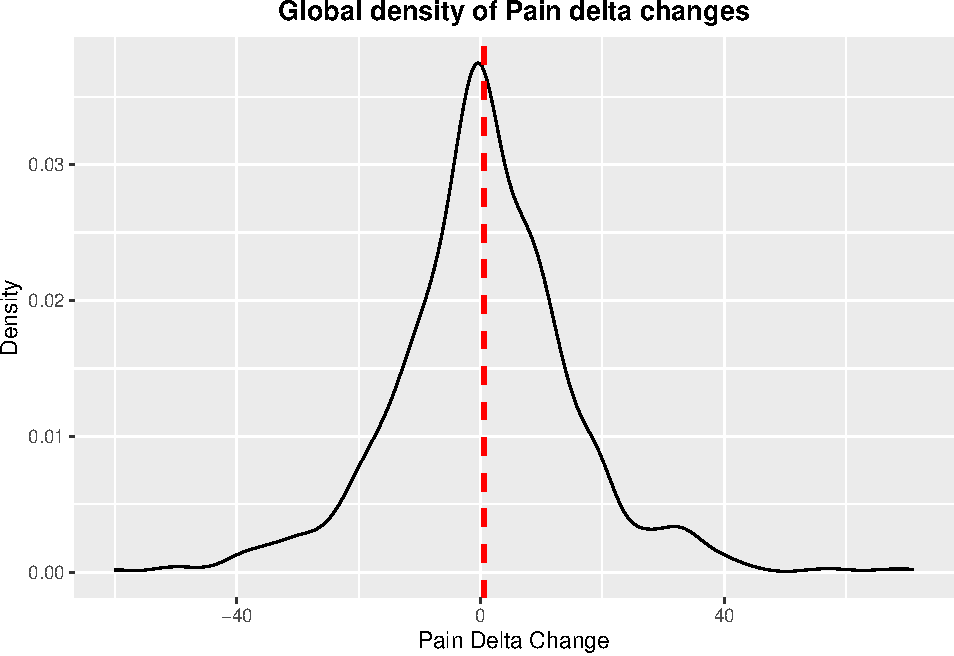
\includegraphics{Martel-Paper_files/figure-latex/unnamed-chunk-15-1.pdf}

\begin{Shaded}
\begin{Highlighting}[]
\DocumentationTok{\#\# Shapiro test (Formal test of normality)}
\NormalTok{normal\_check }\OtherTok{\textless{}{-}}\NormalTok{ data\_paper2}\SpecialCharTok{$}\NormalTok{IndexLev1\_PainAverage\_RawChange[}\SpecialCharTok{!}\FunctionTok{is.na}\NormalTok{(data\_paper2}\SpecialCharTok{$}\NormalTok{IndexLev1\_PainAverage\_RawChange)]}
\FunctionTok{shapiro.test}\NormalTok{(normal\_check) }\CommentTok{\# Although the formal test does not suggest normality}
\end{Highlighting}
\end{Shaded}

\begin{verbatim}
## 
##  Shapiro-Wilk normality test
## 
## data:  normal_check
## W = 0.97198, p-value = 2.216e-11
\end{verbatim}

The below will examine if baseline covairates are associated with the
delta pain change individually.

\begin{Shaded}
\begin{Highlighting}[]
\DocumentationTok{\#\# Age}
\NormalTok{model\_age }\OtherTok{\textless{}{-}} \FunctionTok{lmer}\NormalTok{(IndexLev1\_PainAverage\_RawChange }\SpecialCharTok{\textasciitilde{}}\NormalTok{ Baseline\_Demog\_Age }\SpecialCharTok{+}\NormalTok{ (}\DecValTok{1}\SpecialCharTok{|}\NormalTok{ID), }\AttributeTok{data =}\NormalTok{ data\_paper2)}
\end{Highlighting}
\end{Shaded}

\begin{verbatim}
## boundary (singular) fit: see help('isSingular')
\end{verbatim}

\begin{Shaded}
\begin{Highlighting}[]
\FunctionTok{summary}\NormalTok{(model\_age)}
\end{Highlighting}
\end{Shaded}

\begin{verbatim}
## Linear mixed model fit by REML. t-tests use Satterthwaite's method [
## lmerModLmerTest]
## Formula: IndexLev1_PainAverage_RawChange ~ Baseline_Demog_Age + (1 | ID)
##    Data: data_paper2
## 
## REML criterion at convergence: 6634.2
## 
## Scaled residuals: 
##     Min      1Q  Median      3Q     Max 
## -4.1109 -0.5294 -0.0235  0.5383  4.7535 
## 
## Random effects:
##  Groups   Name        Variance Std.Dev.
##  ID       (Intercept)   0.0     0.00   
##  Residual             221.8    14.89   
## Number of obs: 805, groups:  ID, 155
## 
## Fixed effects:
##                     Estimate Std. Error        df t value Pr(>|t|)
## (Intercept)          3.80726    4.14557 803.00000   0.918    0.359
## Baseline_Demog_Age  -0.04870    0.06225 803.00000  -0.782    0.434
## 
## Correlation of Fixed Effects:
##             (Intr)
## Bsln_Dmg_Ag -0.992
## optimizer (nloptwrap) convergence code: 0 (OK)
## boundary (singular) fit: see help('isSingular')
\end{verbatim}

\begin{Shaded}
\begin{Highlighting}[]
\DocumentationTok{\#\# Sex}
\NormalTok{model\_sex }\OtherTok{\textless{}{-}} \FunctionTok{lmer}\NormalTok{(IndexLev1\_PainAverage\_RawChange }\SpecialCharTok{\textasciitilde{}}\NormalTok{ Baseline\_Demog\_Sex }\SpecialCharTok{+}\NormalTok{ (}\DecValTok{1}\SpecialCharTok{|}\NormalTok{ID), }\AttributeTok{data =}\NormalTok{ data\_paper2)}
\end{Highlighting}
\end{Shaded}

\begin{verbatim}
## boundary (singular) fit: see help('isSingular')
\end{verbatim}

\begin{Shaded}
\begin{Highlighting}[]
\FunctionTok{summary}\NormalTok{(model\_sex)}
\end{Highlighting}
\end{Shaded}

\begin{verbatim}
## Linear mixed model fit by REML. t-tests use Satterthwaite's method [
## lmerModLmerTest]
## Formula: IndexLev1_PainAverage_RawChange ~ Baseline_Demog_Sex + (1 | ID)
##    Data: data_paper2
## 
## REML criterion at convergence: 6693.8
## 
## Scaled residuals: 
##     Min      1Q  Median      3Q     Max 
## -4.0760 -0.5161 -0.0313  0.5586  4.7231 
## 
## Random effects:
##  Groups   Name        Variance Std.Dev.
##  ID       (Intercept)   0.0     0.00   
##  Residual             221.6    14.89   
## Number of obs: 813, groups:  ID, 157
## 
## Fixed effects:
##                    Estimate Std. Error       df t value Pr(>|t|)
## (Intercept)          0.2498     1.7464 811.0000   0.143    0.886
## Baseline_Demog_Sex   0.2168     1.0568 811.0000   0.205    0.838
## 
## Correlation of Fixed Effects:
##             (Intr)
## Bsln_Dmg_Sx -0.954
## optimizer (nloptwrap) convergence code: 0 (OK)
## boundary (singular) fit: see help('isSingular')
\end{verbatim}

\begin{Shaded}
\begin{Highlighting}[]
\DocumentationTok{\#\# BMI}
\NormalTok{model\_bmi }\OtherTok{\textless{}{-}} \FunctionTok{lmer}\NormalTok{(IndexLev1\_PainAverage\_RawChange }\SpecialCharTok{\textasciitilde{}}\NormalTok{ Baseline\_Demog\_BMI }\SpecialCharTok{+}\NormalTok{ (}\DecValTok{1}\SpecialCharTok{|}\NormalTok{ID), }\AttributeTok{data =}\NormalTok{ data\_paper2)}
\end{Highlighting}
\end{Shaded}

\begin{verbatim}
## boundary (singular) fit: see help('isSingular')
\end{verbatim}

\begin{Shaded}
\begin{Highlighting}[]
\FunctionTok{summary}\NormalTok{(model\_bmi)}
\end{Highlighting}
\end{Shaded}

\begin{verbatim}
## Linear mixed model fit by REML. t-tests use Satterthwaite's method [
## lmerModLmerTest]
## Formula: IndexLev1_PainAverage_RawChange ~ Baseline_Demog_BMI + (1 | ID)
##    Data: data_paper2
## 
## REML criterion at convergence: 6548.7
## 
## Scaled residuals: 
##     Min      1Q  Median      3Q     Max 
## -4.0854 -0.5285 -0.0161  0.5370  4.6831 
## 
## Random effects:
##  Groups   Name        Variance Std.Dev.
##  ID       (Intercept)   0.0     0.00   
##  Residual             225.8    15.03   
## Number of obs: 793, groups:  ID, 153
## 
## Fixed effects:
##                     Estimate Std. Error        df t value Pr(>|t|)
## (Intercept)         -2.55505    2.70231 791.00000  -0.946    0.345
## Baseline_Demog_BMI   0.10209    0.08595 791.00000   1.188    0.235
## 
## Correlation of Fixed Effects:
##             (Intr)
## Bsln_Dm_BMI -0.980
## optimizer (nloptwrap) convergence code: 0 (OK)
## boundary (singular) fit: see help('isSingular')
\end{verbatim}

\begin{Shaded}
\begin{Highlighting}[]
\DocumentationTok{\#\# Ethnicity}
\NormalTok{model\_ethn }\OtherTok{\textless{}{-}} \FunctionTok{lmer}\NormalTok{(IndexLev1\_PainAverage\_RawChange }\SpecialCharTok{\textasciitilde{}}\NormalTok{ Baseline\_Demog\_Ethnicity\_Rec }\SpecialCharTok{+}\NormalTok{ (}\DecValTok{1}\SpecialCharTok{|}\NormalTok{ID), }\AttributeTok{data =}\NormalTok{ data\_paper2)}
\end{Highlighting}
\end{Shaded}

\begin{verbatim}
## boundary (singular) fit: see help('isSingular')
\end{verbatim}

\begin{Shaded}
\begin{Highlighting}[]
\FunctionTok{summary}\NormalTok{(model\_ethn)}
\end{Highlighting}
\end{Shaded}

\begin{verbatim}
## Linear mixed model fit by REML. t-tests use Satterthwaite's method [
## lmerModLmerTest]
## Formula: IndexLev1_PainAverage_RawChange ~ Baseline_Demog_Ethnicity_Rec +  
##     (1 | ID)
##    Data: data_paper2
## 
## REML criterion at convergence: 5707.2
## 
## Scaled residuals: 
##     Min      1Q  Median      3Q     Max 
## -4.0600 -0.5292 -0.0100  0.5367  4.6671 
## 
## Random effects:
##  Groups   Name        Variance Std.Dev.
##  ID       (Intercept)   0.0     0.00   
##  Residual             225.3    15.01   
## Number of obs: 692, groups:  ID, 132
## 
## Fixed effects:
##                              Estimate Std. Error       df t value Pr(>|t|)
## (Intercept)                   -0.1436     1.4936 690.0000  -0.096    0.923
## Baseline_Demog_Ethnicity_Rec   1.0869     1.6162 690.0000   0.672    0.502
## 
## Correlation of Fixed Effects:
##             (Intr)
## Bsln_Dm_E_R -0.924
## optimizer (nloptwrap) convergence code: 0 (OK)
## boundary (singular) fit: see help('isSingular')
\end{verbatim}

\begin{Shaded}
\begin{Highlighting}[]
\DocumentationTok{\#\# SmokePerday}
\NormalTok{model\_smoke }\OtherTok{\textless{}{-}} \FunctionTok{lmer}\NormalTok{(IndexLev1\_PainAverage\_RawChange }\SpecialCharTok{\textasciitilde{}}\NormalTok{ Baseline\_Lifestyle\_SmokePerday }\SpecialCharTok{+}\NormalTok{ (}\DecValTok{1}\SpecialCharTok{|}\NormalTok{ID), }\AttributeTok{data =}\NormalTok{ data\_paper2)}
\end{Highlighting}
\end{Shaded}

\begin{verbatim}
## boundary (singular) fit: see help('isSingular')
\end{verbatim}

\begin{Shaded}
\begin{Highlighting}[]
\FunctionTok{summary}\NormalTok{(model\_smoke)}
\end{Highlighting}
\end{Shaded}

\begin{verbatim}
## Linear mixed model fit by REML. t-tests use Satterthwaite's method [
## lmerModLmerTest]
## Formula: IndexLev1_PainAverage_RawChange ~ Baseline_Lifestyle_SmokePerday +  
##     (1 | ID)
##    Data: data_paper2
## 
## REML criterion at convergence: 6698.1
## 
## Scaled residuals: 
##     Min      1Q  Median      3Q     Max 
## -4.0891 -0.5485 -0.0105  0.5275  4.7640 
## 
## Random effects:
##  Groups   Name        Variance Std.Dev.
##  ID       (Intercept)   0.0     0.00   
##  Residual             221.1    14.87   
## Number of obs: 813, groups:  ID, 157
## 
## Fixed effects:
##                                 Estimate Std. Error        df t value Pr(>|t|)
## (Intercept)                      0.15585    0.60882 811.00000   0.256    0.798
## Baseline_Lifestyle_SmokePerday   0.06520    0.04699 811.00000   1.387    0.166
## 
## Correlation of Fixed Effects:
##             (Intr)
## Bsln_Lfs_SP -0.516
## optimizer (nloptwrap) convergence code: 0 (OK)
## boundary (singular) fit: see help('isSingular')
\end{verbatim}

\begin{Shaded}
\begin{Highlighting}[]
\DocumentationTok{\#\# Meds\_Acetaminophen}
\NormalTok{model\_acetam }\OtherTok{\textless{}{-}} \FunctionTok{lmer}\NormalTok{(IndexLev1\_PainAverage\_RawChange }\SpecialCharTok{\textasciitilde{}}\NormalTok{ Baseline\_Meds\_Acetaminophen }\SpecialCharTok{+}\NormalTok{ (}\DecValTok{1}\SpecialCharTok{|}\NormalTok{ID), }\AttributeTok{data =}\NormalTok{ data\_paper2)}
\end{Highlighting}
\end{Shaded}

\begin{verbatim}
## boundary (singular) fit: see help('isSingular')
\end{verbatim}

\begin{Shaded}
\begin{Highlighting}[]
\FunctionTok{summary}\NormalTok{(model\_acetam)}
\end{Highlighting}
\end{Shaded}

\begin{verbatim}
## Linear mixed model fit by REML. t-tests use Satterthwaite's method [
## lmerModLmerTest]
## Formula: IndexLev1_PainAverage_RawChange ~ Baseline_Meds_Acetaminophen +  
##     (1 | ID)
##    Data: data_paper2
## 
## REML criterion at convergence: 6059.2
## 
## Scaled residuals: 
##     Min      1Q  Median      3Q     Max 
## -4.1575 -0.5174 -0.0367  0.5367  4.8396 
## 
## Random effects:
##  Groups   Name        Variance Std.Dev.
##  ID       (Intercept)   0       0.00   
##  Residual             212      14.56   
## Number of obs: 740, groups:  ID, 141
## 
## Fixed effects:
##                             Estimate Std. Error       df t value Pr(>|t|)
## (Intercept)                   0.5342     0.6531 738.0000   0.818    0.414
## Baseline_Meds_Acetaminophen  -0.1309     1.1397 738.0000  -0.115    0.909
## 
## Correlation of Fixed Effects:
##             (Intr)
## Bsln_Mds_Ac -0.573
## optimizer (nloptwrap) convergence code: 0 (OK)
## boundary (singular) fit: see help('isSingular')
\end{verbatim}

\begin{Shaded}
\begin{Highlighting}[]
\DocumentationTok{\#\# NSAID}
\NormalTok{model\_NSAID }\OtherTok{\textless{}{-}} \FunctionTok{lmer}\NormalTok{(IndexLev1\_PainAverage\_RawChange }\SpecialCharTok{\textasciitilde{}}\NormalTok{ Baseline\_Meds\_NSAID }\SpecialCharTok{+}\NormalTok{ (}\DecValTok{1}\SpecialCharTok{|}\NormalTok{ID), }\AttributeTok{data =}\NormalTok{ data\_paper2)}
\end{Highlighting}
\end{Shaded}

\begin{verbatim}
## boundary (singular) fit: see help('isSingular')
\end{verbatim}

\begin{Shaded}
\begin{Highlighting}[]
\FunctionTok{summary}\NormalTok{(model\_NSAID)}
\end{Highlighting}
\end{Shaded}

\begin{verbatim}
## Linear mixed model fit by REML. t-tests use Satterthwaite's method [
## lmerModLmerTest]
## Formula: IndexLev1_PainAverage_RawChange ~ Baseline_Meds_NSAID + (1 |      ID)
##    Data: data_paper2
## 
## REML criterion at convergence: 6105
## 
## Scaled residuals: 
##     Min      1Q  Median      3Q     Max 
## -4.1942 -0.4919 -0.0100  0.5561  4.8245 
## 
## Random effects:
##  Groups   Name        Variance Std.Dev.
##  ID       (Intercept)   0       0.00   
##  Residual             211      14.53   
## Number of obs: 746, groups:  ID, 142
## 
## Fixed effects:
##                     Estimate Std. Error       df t value Pr(>|t|)
## (Intercept)           0.9221     0.7593 744.0000   1.215    0.225
## Baseline_Meds_NSAID  -0.7774     1.0638 744.0000  -0.731    0.465
## 
## Correlation of Fixed Effects:
##             (Intr)
## Bsl_M_NSAID -0.714
## optimizer (nloptwrap) convergence code: 0 (OK)
## boundary (singular) fit: see help('isSingular')
\end{verbatim}

\begin{Shaded}
\begin{Highlighting}[]
\DocumentationTok{\#\# Cox2}
\NormalTok{model\_cox2 }\OtherTok{\textless{}{-}} \FunctionTok{lmer}\NormalTok{(IndexLev1\_PainAverage\_RawChange }\SpecialCharTok{\textasciitilde{}}\NormalTok{ Baseline\_Meds\_Cox2 }\SpecialCharTok{+}\NormalTok{ (}\DecValTok{1}\SpecialCharTok{|}\NormalTok{ID), }\AttributeTok{data =}\NormalTok{ data\_paper2)}
\end{Highlighting}
\end{Shaded}

\begin{verbatim}
## boundary (singular) fit: see help('isSingular')
\end{verbatim}

\begin{Shaded}
\begin{Highlighting}[]
\FunctionTok{summary}\NormalTok{(model\_cox2)}
\end{Highlighting}
\end{Shaded}

\begin{verbatim}
## Linear mixed model fit by REML. t-tests use Satterthwaite's method [
## lmerModLmerTest]
## Formula: IndexLev1_PainAverage_RawChange ~ Baseline_Meds_Cox2 + (1 | ID)
##    Data: data_paper2
## 
## REML criterion at convergence: 6103
## 
## Scaled residuals: 
##     Min      1Q  Median      3Q     Max 
## -4.1660 -0.5185 -0.0367  0.5827  4.8495 
## 
## Random effects:
##  Groups   Name        Variance Std.Dev.
##  ID       (Intercept)   0.0     0.00   
##  Residual             211.1    14.53   
## Number of obs: 746, groups:  ID, 142
## 
## Fixed effects:
##                    Estimate Std. Error       df t value Pr(>|t|)
## (Intercept)          0.5336     0.5378 744.0000   0.992    0.321
## Baseline_Meds_Cox2  -0.3461     3.6722 744.0000  -0.094    0.925
## 
## Correlation of Fixed Effects:
##             (Intr)
## Bsln_Mds_C2 -0.146
## optimizer (nloptwrap) convergence code: 0 (OK)
## boundary (singular) fit: see help('isSingular')
\end{verbatim}

\begin{Shaded}
\begin{Highlighting}[]
\DocumentationTok{\#\# Antidepressants}
\NormalTok{model\_antidep }\OtherTok{\textless{}{-}} \FunctionTok{lmer}\NormalTok{(IndexLev1\_PainAverage\_RawChange }\SpecialCharTok{\textasciitilde{}}\NormalTok{ Baseline\_Meds\_Antidepressants }\SpecialCharTok{+}\NormalTok{ (}\DecValTok{1}\SpecialCharTok{|}\NormalTok{ID), }\AttributeTok{data =}\NormalTok{ data\_paper2)}
\end{Highlighting}
\end{Shaded}

\begin{verbatim}
## boundary (singular) fit: see help('isSingular')
\end{verbatim}

\begin{Shaded}
\begin{Highlighting}[]
\FunctionTok{summary}\NormalTok{(model\_antidep)}
\end{Highlighting}
\end{Shaded}

\begin{verbatim}
## Linear mixed model fit by REML. t-tests use Satterthwaite's method [
## lmerModLmerTest]
## Formula: IndexLev1_PainAverage_RawChange ~ Baseline_Meds_Antidepressants +  
##     (1 | ID)
##    Data: data_paper2
## 
## REML criterion at convergence: 6104.3
## 
## Scaled residuals: 
##     Min      1Q  Median      3Q     Max 
## -4.1600 -0.5119 -0.0301  0.5326  4.8569 
## 
## Random effects:
##  Groups   Name        Variance Std.Dev.
##  ID       (Intercept)   0.0     0.00   
##  Residual             211.1    14.53   
## Number of obs: 746, groups:  ID, 142
## 
## Fixed effects:
##                               Estimate Std. Error       df t value Pr(>|t|)
## (Intercept)                     0.4377     0.5630 744.0000   0.777    0.437
## Baseline_Meds_Antidepressants   0.8248     1.7191 744.0000   0.480    0.632
## 
## Correlation of Fixed Effects:
##             (Intr)
## Bsln_Mds_An -0.327
## optimizer (nloptwrap) convergence code: 0 (OK)
## boundary (singular) fit: see help('isSingular')
\end{verbatim}

\begin{Shaded}
\begin{Highlighting}[]
\DocumentationTok{\#\# Baseline\_Meds\_Anxiolytics}
\NormalTok{model\_anxioly }\OtherTok{\textless{}{-}} \FunctionTok{lmer}\NormalTok{(IndexLev1\_PainAverage\_RawChange }\SpecialCharTok{\textasciitilde{}}\NormalTok{ Baseline\_Meds\_Anxiolytics }\SpecialCharTok{+}\NormalTok{ (}\DecValTok{1}\SpecialCharTok{|}\NormalTok{ID), }\AttributeTok{data =}\NormalTok{ data\_paper2)}
\end{Highlighting}
\end{Shaded}

\begin{verbatim}
## boundary (singular) fit: see help('isSingular')
\end{verbatim}

\begin{Shaded}
\begin{Highlighting}[]
\FunctionTok{summary}\NormalTok{(model\_anxioly)}
\end{Highlighting}
\end{Shaded}

\begin{verbatim}
## Linear mixed model fit by REML. t-tests use Satterthwaite's method [
## lmerModLmerTest]
## Formula: IndexLev1_PainAverage_RawChange ~ Baseline_Meds_Anxiolytics +  
##     (1 | ID)
##    Data: data_paper2
## 
## REML criterion at convergence: 6104
## 
## Scaled residuals: 
##     Min      1Q  Median      3Q     Max 
## -4.1661 -0.5186 -0.0369  0.5825  4.8494 
## 
## Random effects:
##  Groups   Name        Variance Std.Dev.
##  ID       (Intercept)   0.0     0.00   
##  Residual             211.1    14.53   
## Number of obs: 746, groups:  ID, 142
## 
## Fixed effects:
##                           Estimate Std. Error       df t value Pr(>|t|)
## (Intercept)                 0.5357     0.5488 744.0000   0.976    0.329
## Baseline_Meds_Anxiolytics  -0.1579     2.2345 744.0000  -0.071    0.944
## 
## Correlation of Fixed Effects:
##             (Intr)
## Bsln_Mds_An -0.246
## optimizer (nloptwrap) convergence code: 0 (OK)
## boundary (singular) fit: see help('isSingular')
\end{verbatim}

\begin{Shaded}
\begin{Highlighting}[]
\DocumentationTok{\#\# MuscleRelaxants}
\NormalTok{model\_musclerelax }\OtherTok{\textless{}{-}} \FunctionTok{lmer}\NormalTok{(IndexLev1\_PainAverage\_RawChange }\SpecialCharTok{\textasciitilde{}}\NormalTok{ Baseline\_Meds\_MuscleRelaxants }\SpecialCharTok{+}\NormalTok{ (}\DecValTok{1}\SpecialCharTok{|}\NormalTok{ID), }\AttributeTok{data =}\NormalTok{ data\_paper2)}
\end{Highlighting}
\end{Shaded}

\begin{verbatim}
## boundary (singular) fit: see help('isSingular')
\end{verbatim}

\begin{Shaded}
\begin{Highlighting}[]
\FunctionTok{summary}\NormalTok{(model\_musclerelax)}
\end{Highlighting}
\end{Shaded}

\begin{verbatim}
## Linear mixed model fit by REML. t-tests use Satterthwaite's method [
## lmerModLmerTest]
## Formula: IndexLev1_PainAverage_RawChange ~ Baseline_Meds_MuscleRelaxants +  
##     (1 | ID)
##    Data: data_paper2
## 
## REML criterion at convergence: 6103.9
## 
## Scaled residuals: 
##     Min      1Q  Median      3Q     Max 
## -4.1713 -0.5232 -0.0414  0.5781  4.9182 
## 
## Random effects:
##  Groups   Name        Variance Std.Dev.
##  ID       (Intercept)   0.0     0.00   
##  Residual             211.1    14.53   
## Number of obs: 746, groups:  ID, 142
## 
## Fixed effects:
##                               Estimate Std. Error       df t value Pr(>|t|)
## (Intercept)                     0.6010     0.5519 744.0000   1.089    0.276
## Baseline_Meds_MuscleRelaxants  -1.0538     2.0705 744.0000  -0.509    0.611
## 
## Correlation of Fixed Effects:
##             (Intr)
## Bsln_Mds_MR -0.267
## optimizer (nloptwrap) convergence code: 0 (OK)
## boundary (singular) fit: see help('isSingular')
\end{verbatim}

\begin{Shaded}
\begin{Highlighting}[]
\DocumentationTok{\#\# Baseline\_Meds\_Opioids}
\NormalTok{model\_opioid }\OtherTok{\textless{}{-}} \FunctionTok{lmer}\NormalTok{(IndexLev1\_PainAverage\_RawChange }\SpecialCharTok{\textasciitilde{}}\NormalTok{ Baseline\_Meds\_Opioids }\SpecialCharTok{+}\NormalTok{ (}\DecValTok{1}\SpecialCharTok{|}\NormalTok{ID), }\AttributeTok{data =}\NormalTok{ data\_paper2)}
\end{Highlighting}
\end{Shaded}

\begin{verbatim}
## boundary (singular) fit: see help('isSingular')
\end{verbatim}

\begin{Shaded}
\begin{Highlighting}[]
\FunctionTok{summary}\NormalTok{(model\_opioid)}
\end{Highlighting}
\end{Shaded}

\begin{verbatim}
## Linear mixed model fit by REML. t-tests use Satterthwaite's method [
## lmerModLmerTest]
## Formula: IndexLev1_PainAverage_RawChange ~ Baseline_Meds_Opioids + (1 |  
##     ID)
##    Data: data_paper2
## 
## REML criterion at convergence: 6104.4
## 
## Scaled residuals: 
##     Min      1Q  Median      3Q     Max 
## -4.1636 -0.5181 -0.0364  0.5830  4.8498 
## 
## Random effects:
##  Groups   Name        Variance Std.Dev.
##  ID       (Intercept)   0.0     0.00   
##  Residual             211.1    14.53   
## Number of obs: 746, groups:  ID, 142
## 
## Fixed effects:
##                        Estimate Std. Error        df t value Pr(>|t|)
## (Intercept)             0.52868    0.55722 744.00000   0.949    0.343
## Baseline_Meds_Opioids  -0.02868    1.87339 744.00000  -0.015    0.988
## 
## Correlation of Fixed Effects:
##             (Intr)
## Bsln_Mds_Op -0.297
## optimizer (nloptwrap) convergence code: 0 (OK)
## boundary (singular) fit: see help('isSingular')
\end{verbatim}

\begin{Shaded}
\begin{Highlighting}[]
\DocumentationTok{\#\# Baseline\_Meds\_Anticonvulsants}
\NormalTok{model\_anticonv }\OtherTok{\textless{}{-}} \FunctionTok{lmer}\NormalTok{(IndexLev1\_PainAverage\_RawChange }\SpecialCharTok{\textasciitilde{}}\NormalTok{ Baseline\_Meds\_Anticonvulsants }\SpecialCharTok{+}\NormalTok{ (}\DecValTok{1}\SpecialCharTok{|}\NormalTok{ID), }\AttributeTok{data =}\NormalTok{ data\_paper2)}
\end{Highlighting}
\end{Shaded}

\begin{verbatim}
## boundary (singular) fit: see help('isSingular')
\end{verbatim}

\begin{Shaded}
\begin{Highlighting}[]
\FunctionTok{summary}\NormalTok{(model\_anticonv)}
\end{Highlighting}
\end{Shaded}

\begin{verbatim}
## Linear mixed model fit by REML. t-tests use Satterthwaite's method [
## lmerModLmerTest]
## Formula: IndexLev1_PainAverage_RawChange ~ Baseline_Meds_Anticonvulsants +  
##     (1 | ID)
##    Data: data_paper2
## 
## REML criterion at convergence: 6103.3
## 
## Scaled residuals: 
##     Min      1Q  Median      3Q     Max 
## -4.1654 -0.5180 -0.0362  0.5832  4.8500 
## 
## Random effects:
##  Groups   Name        Variance Std.Dev.
##  ID       (Intercept)   0.0     0.00   
##  Residual             211.1    14.53   
## Number of obs: 746, groups:  ID, 142
## 
## Fixed effects:
##                                 Estimate Std. Error         df t value Pr(>|t|)
## (Intercept)                     0.526207   0.539654 744.000000   0.975    0.330
## Baseline_Meds_Anticonvulsants  -0.002397   3.216440 744.000000  -0.001    0.999
## 
## Correlation of Fixed Effects:
##             (Intr)
## Bsln_Mds_An -0.168
## optimizer (nloptwrap) convergence code: 0 (OK)
## boundary (singular) fit: see help('isSingular')
\end{verbatim}

\hypertarget{level-2-covariates}{%
\subsection{Level 2 covariates}\label{level-2-covariates}}

The below will examine if PPTh, TSP, and CPM are significantly
associated with the delta pain change.

\begin{Shaded}
\begin{Highlighting}[]
\DocumentationTok{\#\# PPTh}
\NormalTok{model\_PPTh }\OtherTok{\textless{}{-}} \FunctionTok{lmer}\NormalTok{(IndexLev1\_PainAverage\_RawChange }\SpecialCharTok{\textasciitilde{}}\NormalTok{ IndexLev2\_QST\_BaselinePPTh }\SpecialCharTok{+}\NormalTok{ (}\DecValTok{1}\SpecialCharTok{|}\NormalTok{ID), }\AttributeTok{data =}\NormalTok{ data\_paper2)}
\end{Highlighting}
\end{Shaded}

\begin{verbatim}
## boundary (singular) fit: see help('isSingular')
\end{verbatim}

\begin{Shaded}
\begin{Highlighting}[]
\FunctionTok{summary}\NormalTok{(model\_PPTh)}
\end{Highlighting}
\end{Shaded}

\begin{verbatim}
## Linear mixed model fit by REML. t-tests use Satterthwaite's method [
## lmerModLmerTest]
## Formula: IndexLev1_PainAverage_RawChange ~ IndexLev2_QST_BaselinePPTh +  
##     (1 | ID)
##    Data: data_paper2
## 
## REML criterion at convergence: 6035.7
## 
## Scaled residuals: 
##     Min      1Q  Median      3Q     Max 
## -4.0198 -0.5541 -0.0301  0.5472  4.6470 
## 
## Random effects:
##  Groups   Name        Variance Std.Dev.
##  ID       (Intercept)   0.0     0.00   
##  Residual             228.5    15.12   
## Number of obs: 729, groups:  ID, 142
## 
## Fixed effects:
##                              Estimate Std. Error         df t value Pr(>|t|)
## (Intercept)                  0.999941   1.202766 727.000000   0.831    0.406
## IndexLev2_QST_BaselinePPTh  -0.001204   0.002685 727.000000  -0.448    0.654
## 
## Correlation of Fixed Effects:
##             (Intr)
## IL2_QST_BPP -0.885
## optimizer (nloptwrap) convergence code: 0 (OK)
## boundary (singular) fit: see help('isSingular')
\end{verbatim}

\begin{Shaded}
\begin{Highlighting}[]
\DocumentationTok{\#\# TSP }
\NormalTok{model\_TSP }\OtherTok{\textless{}{-}} \FunctionTok{lmer}\NormalTok{(IndexLev1\_PainAverage\_RawChange }\SpecialCharTok{\textasciitilde{}}\NormalTok{ IndexLev2\_QST\_TSPAve }\SpecialCharTok{+}\NormalTok{ (}\DecValTok{1}\SpecialCharTok{|}\NormalTok{ID), }\AttributeTok{data =}\NormalTok{ data\_paper2)}
\end{Highlighting}
\end{Shaded}

\begin{verbatim}
## boundary (singular) fit: see help('isSingular')
\end{verbatim}

\begin{Shaded}
\begin{Highlighting}[]
\FunctionTok{summary}\NormalTok{(model\_TSP)}
\end{Highlighting}
\end{Shaded}

\begin{verbatim}
## Linear mixed model fit by REML. t-tests use Satterthwaite's method [
## lmerModLmerTest]
## Formula: IndexLev1_PainAverage_RawChange ~ IndexLev2_QST_TSPAve + (1 |      ID)
##    Data: data_paper2
## 
## REML criterion at convergence: 6283.5
## 
## Scaled residuals: 
##     Min      1Q  Median      3Q     Max 
## -4.0486 -0.5141 -0.0379  0.5535  4.6865 
## 
## Random effects:
##  Groups   Name        Variance Std.Dev.
##  ID       (Intercept)   0.0     0      
##  Residual             224.9    15      
## Number of obs: 761, groups:  ID, 146
## 
## Fixed effects:
##                       Estimate Std. Error        df t value Pr(>|t|)
## (Intercept)            0.71948    0.67826 759.00000   1.061    0.289
## IndexLev2_QST_TSPAve  -0.01010    0.02899 759.00000  -0.348    0.728
## 
## Correlation of Fixed Effects:
##             (Intr)
## IL2_QST_TSP -0.598
## optimizer (nloptwrap) convergence code: 0 (OK)
## boundary (singular) fit: see help('isSingular')
\end{verbatim}

\begin{Shaded}
\begin{Highlighting}[]
\DocumentationTok{\#\# CPM}
\NormalTok{model\_CPM }\OtherTok{\textless{}{-}} \FunctionTok{lmer}\NormalTok{(IndexLev1\_PainAverage\_RawChange }\SpecialCharTok{\textasciitilde{}}\NormalTok{ IndexLev2\_QST\_CpmTrialAve }\SpecialCharTok{+}\NormalTok{ (}\DecValTok{1}\SpecialCharTok{|}\NormalTok{ID), }\AttributeTok{data =}\NormalTok{ data\_paper2)}
\end{Highlighting}
\end{Shaded}

\begin{verbatim}
## boundary (singular) fit: see help('isSingular')
\end{verbatim}

\begin{Shaded}
\begin{Highlighting}[]
\FunctionTok{summary}\NormalTok{(model\_CPM)}
\end{Highlighting}
\end{Shaded}

\begin{verbatim}
## Linear mixed model fit by REML. t-tests use Satterthwaite's method [
## lmerModLmerTest]
## Formula: IndexLev1_PainAverage_RawChange ~ IndexLev2_QST_CpmTrialAve +  
##     (1 | ID)
##    Data: data_paper2
## 
## REML criterion at convergence: 5966.9
## 
## Scaled residuals: 
##     Min      1Q  Median      3Q     Max 
## -4.0278 -0.5057 -0.0370  0.5571  4.6857 
## 
## Random effects:
##  Groups   Name        Variance Std.Dev.
##  ID       (Intercept)   0.0     0.00   
##  Residual             226.3    15.04   
## Number of obs: 722, groups:  ID, 141
## 
## Fixed effects:
##                             Estimate Std. Error         df t value Pr(>|t|)
## (Intercept)                 0.881281   2.276000 720.000000   0.387    0.699
## IndexLev2_QST_CpmTrialAve  -0.002652   0.017876 720.000000  -0.148    0.882
## 
## Correlation of Fixed Effects:
##             (Intr)
## IL2_QST_CTA -0.969
## optimizer (nloptwrap) convergence code: 0 (OK)
## boundary (singular) fit: see help('isSingular')
\end{verbatim}

\begin{Shaded}
\begin{Highlighting}[]
\DocumentationTok{\#\# Adjusted model}
\NormalTok{model\_adjusted\_lev2 }\OtherTok{\textless{}{-}} \FunctionTok{lmer}\NormalTok{(IndexLev1\_PainAverage\_RawChange }\SpecialCharTok{\textasciitilde{}}\NormalTok{ IndexLev2\_QST\_CpmTrialAve }\SpecialCharTok{+}\NormalTok{ IndexLev2\_QST\_TSPAve }\SpecialCharTok{+}\NormalTok{ IndexLev2\_QST\_BaselinePPTh }\SpecialCharTok{+}\NormalTok{ (}\DecValTok{1}\SpecialCharTok{|}\NormalTok{ID), }\AttributeTok{data =}\NormalTok{ data\_paper2)}
\end{Highlighting}
\end{Shaded}

\begin{verbatim}
## boundary (singular) fit: see help('isSingular')
\end{verbatim}

\begin{Shaded}
\begin{Highlighting}[]
\FunctionTok{summary}\NormalTok{(model\_adjusted\_lev2)}
\end{Highlighting}
\end{Shaded}

\begin{verbatim}
## Linear mixed model fit by REML. t-tests use Satterthwaite's method [
## lmerModLmerTest]
## Formula: IndexLev1_PainAverage_RawChange ~ IndexLev2_QST_CpmTrialAve +  
##     IndexLev2_QST_TSPAve + IndexLev2_QST_BaselinePPTh + (1 |      ID)
##    Data: data_paper2
## 
## REML criterion at convergence: 5683.2
## 
## Scaled residuals: 
##     Min      1Q  Median      3Q     Max 
## -4.0180 -0.5348 -0.0257  0.5470  4.5886 
## 
## Random effects:
##  Groups   Name        Variance Std.Dev.
##  ID       (Intercept)   0.0     0.00   
##  Residual             232.1    15.23   
## Number of obs: 684, groups:  ID, 132
## 
## Fixed effects:
##                              Estimate Std. Error         df t value Pr(>|t|)
## (Intercept)                  2.139130   3.138091 680.000000   0.682    0.496
## IndexLev2_QST_CpmTrialAve   -0.004746   0.019330 680.000000  -0.246    0.806
## IndexLev2_QST_TSPAve        -0.014221   0.031074 680.000000  -0.458    0.647
## IndexLev2_QST_BaselinePPTh  -0.001967   0.003138 680.000000  -0.627    0.531
## 
## Correlation of Fixed Effects:
##             (Intr) IL2_QST_C IL2_QST_T
## IL2_QST_CTA -0.879                    
## IL2_QST_TSP -0.284  0.056             
## IL2_QST_BPP -0.643  0.277     0.237   
## optimizer (nloptwrap) convergence code: 0 (OK)
## boundary (singular) fit: see help('isSingular')
\end{verbatim}

\hypertarget{level-1-covariates}{%
\subsection{Level 1 covariates}\label{level-1-covariates}}

The following will examine if DailyCatastro, DailyNA, Daily PosAffect,
DailyPhysExcersice are associated with the delta change in pain

\begin{Shaded}
\begin{Highlighting}[]
\DocumentationTok{\#\# Daily Catastro}
\NormalTok{model\_catastro }\OtherTok{\textless{}{-}} \FunctionTok{lmer}\NormalTok{(IndexLev1\_PainAverage\_RawChange }\SpecialCharTok{\textasciitilde{}}\NormalTok{ IndexLev1\_Catastrophizing\_Total }\SpecialCharTok{+}\NormalTok{ (}\DecValTok{1}\SpecialCharTok{|}\NormalTok{ID), }\AttributeTok{data =}\NormalTok{ data\_paper2)}
\end{Highlighting}
\end{Shaded}

\begin{verbatim}
## boundary (singular) fit: see help('isSingular')
\end{verbatim}

\begin{Shaded}
\begin{Highlighting}[]
\FunctionTok{summary}\NormalTok{(model\_catastro) }\CommentTok{\# Significant!}
\end{Highlighting}
\end{Shaded}

\begin{verbatim}
## Linear mixed model fit by REML. t-tests use Satterthwaite's method [
## lmerModLmerTest]
## Formula: IndexLev1_PainAverage_RawChange ~ IndexLev1_Catastrophizing_Total +  
##     (1 | ID)
##    Data: data_paper2
## 
## REML criterion at convergence: 6670.2
## 
## Scaled residuals: 
##     Min      1Q  Median      3Q     Max 
## -4.0629 -0.5571  0.0302  0.5450  4.6436 
## 
## Random effects:
##  Groups   Name        Variance Std.Dev.
##  ID       (Intercept)   0.0     0.00   
##  Residual             215.4    14.68   
## Number of obs: 812, groups:  ID, 157
## 
## Fixed effects:
##                                  Estimate Std. Error        df t value Pr(>|t|)
## (Intercept)                      -1.69145    0.69735 810.00000  -2.426   0.0155
## IndexLev1_Catastrophizing_Total   0.10163    0.02079 810.00000   4.888 1.23e-06
##                                    
## (Intercept)                     *  
## IndexLev1_Catastrophizing_Total ***
## ---
## Signif. codes:  0 '***' 0.001 '**' 0.01 '*' 0.05 '.' 0.1 ' ' 1
## 
## Correlation of Fixed Effects:
##             (Intr)
## IndxLv1_C_T -0.674
## optimizer (nloptwrap) convergence code: 0 (OK)
## boundary (singular) fit: see help('isSingular')
\end{verbatim}

\begin{Shaded}
\begin{Highlighting}[]
\DocumentationTok{\#\# DailyNA}
\NormalTok{model\_DailyNA }\OtherTok{\textless{}{-}} \FunctionTok{lmer}\NormalTok{(IndexLev1\_PainAverage\_RawChange }\SpecialCharTok{\textasciitilde{}}\NormalTok{ IndexLev1\_NegativeAffect\_Total }\SpecialCharTok{+}\NormalTok{ (}\DecValTok{1}\SpecialCharTok{|}\NormalTok{ID), }\AttributeTok{data =}\NormalTok{ data\_paper2)}
\end{Highlighting}
\end{Shaded}

\begin{verbatim}
## boundary (singular) fit: see help('isSingular')
\end{verbatim}

\begin{Shaded}
\begin{Highlighting}[]
\FunctionTok{summary}\NormalTok{(model\_DailyNA) }\CommentTok{\# Significant!}
\end{Highlighting}
\end{Shaded}

\begin{verbatim}
## Linear mixed model fit by REML. t-tests use Satterthwaite's method [
## lmerModLmerTest]
## Formula: IndexLev1_PainAverage_RawChange ~ IndexLev1_NegativeAffect_Total +  
##     (1 | ID)
##    Data: data_paper2
## 
## REML criterion at convergence: 6686.2
## 
## Scaled residuals: 
##     Min      1Q  Median      3Q     Max 
## -4.0924 -0.5408 -0.0025  0.5375  4.6374 
## 
## Random effects:
##  Groups   Name        Variance Std.Dev.
##  ID       (Intercept)   0.0     0.00   
##  Residual             219.8    14.83   
## Number of obs: 812, groups:  ID, 157
## 
## Fixed effects:
##                                 Estimate Std. Error        df t value Pr(>|t|)
## (Intercept)                     -0.92603    0.82773 810.00000  -1.119   0.2636
## IndexLev1_NegativeAffect_Total   0.06144    0.02561 810.00000   2.399   0.0167
##                                 
## (Intercept)                     
## IndexLev1_NegativeAffect_Total *
## ---
## Signif. codes:  0 '***' 0.001 '**' 0.01 '*' 0.05 '.' 0.1 ' ' 1
## 
## Correlation of Fixed Effects:
##             (Intr)
## IndxL1_NA_T -0.778
## optimizer (nloptwrap) convergence code: 0 (OK)
## boundary (singular) fit: see help('isSingular')
\end{verbatim}

\begin{Shaded}
\begin{Highlighting}[]
\DocumentationTok{\#\# PosAffect}
\NormalTok{model\_PosAffect }\OtherTok{\textless{}{-}} \FunctionTok{lmer}\NormalTok{(IndexLev1\_PainAverage\_RawChange }\SpecialCharTok{\textasciitilde{}}\NormalTok{ IndexLev1\_PositiveAffect\_Total }\SpecialCharTok{+}\NormalTok{ (}\DecValTok{1}\SpecialCharTok{|}\NormalTok{ID), }\AttributeTok{data =}\NormalTok{ data\_paper2)}
\end{Highlighting}
\end{Shaded}

\begin{verbatim}
## boundary (singular) fit: see help('isSingular')
\end{verbatim}

\begin{Shaded}
\begin{Highlighting}[]
\FunctionTok{summary}\NormalTok{(model\_PosAffect)}
\end{Highlighting}
\end{Shaded}

\begin{verbatim}
## Linear mixed model fit by REML. t-tests use Satterthwaite's method [
## lmerModLmerTest]
## Formula: IndexLev1_PainAverage_RawChange ~ IndexLev1_PositiveAffect_Total +  
##     (1 | ID)
##    Data: data_paper2
## 
## REML criterion at convergence: 6688.8
## 
## Scaled residuals: 
##     Min      1Q  Median      3Q     Max 
## -4.1242 -0.5363 -0.0145  0.5156  4.6655 
## 
## Random effects:
##  Groups   Name        Variance Std.Dev.
##  ID       (Intercept)   0.0     0.00   
##  Residual             220.5    14.85   
## Number of obs: 812, groups:  ID, 157
## 
## Fixed effects:
##                                 Estimate Std. Error        df t value Pr(>|t|)
## (Intercept)                      3.85909    1.94542 810.00000   1.984   0.0476
## IndexLev1_PositiveAffect_Total  -0.04838    0.02798 810.00000  -1.729   0.0842
##                                 
## (Intercept)                    *
## IndexLev1_PositiveAffect_Total .
## ---
## Signif. codes:  0 '***' 0.001 '**' 0.01 '*' 0.05 '.' 0.1 ' ' 1
## 
## Correlation of Fixed Effects:
##             (Intr)
## IndxL1_PA_T -0.963
## optimizer (nloptwrap) convergence code: 0 (OK)
## boundary (singular) fit: see help('isSingular')
\end{verbatim}

\begin{Shaded}
\begin{Highlighting}[]
\DocumentationTok{\#\# DailyPhysExcersice}
\NormalTok{model\_PhysExercise }\OtherTok{\textless{}{-}} \FunctionTok{lmer}\NormalTok{(IndexLev1\_PainAverage\_RawChange }\SpecialCharTok{\textasciitilde{}}\NormalTok{ Level1\_Even\_PhysActiv }\SpecialCharTok{+}\NormalTok{ (}\DecValTok{1}\SpecialCharTok{|}\NormalTok{ID), }\AttributeTok{data =}\NormalTok{ data\_paper2)}
\end{Highlighting}
\end{Shaded}

\begin{verbatim}
## boundary (singular) fit: see help('isSingular')
\end{verbatim}

\begin{Shaded}
\begin{Highlighting}[]
\FunctionTok{summary}\NormalTok{(model\_PhysExercise) }\CommentTok{\# Significant! }
\end{Highlighting}
\end{Shaded}

\begin{verbatim}
## Linear mixed model fit by REML. t-tests use Satterthwaite's method [
## lmerModLmerTest]
## Formula: IndexLev1_PainAverage_RawChange ~ Level1_Even_PhysActiv + (1 |  
##     ID)
##    Data: data_paper2
## 
## REML criterion at convergence: 6578.2
## 
## Scaled residuals: 
##     Min      1Q  Median      3Q     Max 
## -3.9409 -0.5310 -0.0294  0.5356  4.8044 
## 
## Random effects:
##  Groups   Name        Variance Std.Dev.
##  ID       (Intercept)   0.0     0.00   
##  Residual             221.8    14.89   
## Number of obs: 798, groups:  ID, 154
## 
## Fixed effects:
##                        Estimate Std. Error        df t value Pr(>|t|)  
## (Intercept)            -1.87629    1.26938 796.00000  -1.478   0.1398  
## Level1_Even_PhysActiv   0.05115    0.02374 796.00000   2.154   0.0315 *
## ---
## Signif. codes:  0 '***' 0.001 '**' 0.01 '*' 0.05 '.' 0.1 ' ' 1
## 
## Correlation of Fixed Effects:
##             (Intr)
## Lvl1_Evn_PA -0.910
## optimizer (nloptwrap) convergence code: 0 (OK)
## boundary (singular) fit: see help('isSingular')
\end{verbatim}

\begin{Shaded}
\begin{Highlighting}[]
\DocumentationTok{\#\# Adjusted level 1}
\NormalTok{model\_adj\_lev1 }\OtherTok{\textless{}{-}} \FunctionTok{lmer}\NormalTok{(IndexLev1\_PainAverage\_RawChange }\SpecialCharTok{\textasciitilde{}}\NormalTok{ Level1\_Even\_PhysActiv }\SpecialCharTok{+}\NormalTok{ IndexLev1\_PositiveAffect\_Total }\SpecialCharTok{+}\NormalTok{ IndexLev1\_NegativeAffect\_Total }\SpecialCharTok{+}\NormalTok{ IndexLev1\_Catastrophizing\_Total }\SpecialCharTok{+}\NormalTok{ (}\DecValTok{1}\SpecialCharTok{|}\NormalTok{ID), }\AttributeTok{data =}\NormalTok{ data\_paper2)}
\end{Highlighting}
\end{Shaded}

\begin{verbatim}
## boundary (singular) fit: see help('isSingular')
\end{verbatim}

\begin{Shaded}
\begin{Highlighting}[]
\FunctionTok{summary}\NormalTok{(model\_adj\_lev1) }\CommentTok{\# Catastro significant! }
\end{Highlighting}
\end{Shaded}

\begin{verbatim}
## Linear mixed model fit by REML. t-tests use Satterthwaite's method [
## lmerModLmerTest]
## Formula: 
## IndexLev1_PainAverage_RawChange ~ Level1_Even_PhysActiv + IndexLev1_PositiveAffect_Total +  
##     IndexLev1_NegativeAffect_Total + IndexLev1_Catastrophizing_Total +  
##     (1 | ID)
##    Data: data_paper2
## 
## REML criterion at convergence: 6573.5
## 
## Scaled residuals: 
##     Min      1Q  Median      3Q     Max 
## -3.9903 -0.5522  0.0234  0.5361  4.6724 
## 
## Random effects:
##  Groups   Name        Variance Std.Dev.
##  ID       (Intercept)   0.0     0.00   
##  Residual             216.9    14.73   
## Number of obs: 798, groups:  ID, 154
## 
## Fixed effects:
##                                  Estimate Std. Error        df t value Pr(>|t|)
## (Intercept)                      -1.31483    2.90515 793.00000  -0.453    0.651
## Level1_Even_PhysActiv             0.03084    0.02426 793.00000   1.271    0.204
## IndexLev1_PositiveAffect_Total   -0.02196    0.03421 793.00000  -0.642    0.521
## IndexLev1_NegativeAffect_Total   -0.01274    0.03429 793.00000  -0.372    0.710
## IndexLev1_Catastrophizing_Total   0.09698    0.02478 793.00000   3.914 9.85e-05
##                                    
## (Intercept)                        
## Level1_Even_PhysActiv              
## IndexLev1_PositiveAffect_Total     
## IndexLev1_NegativeAffect_Total     
## IndexLev1_Catastrophizing_Total ***
## ---
## Signif. codes:  0 '***' 0.001 '**' 0.01 '*' 0.05 '.' 0.1 ' ' 1
## 
## Correlation of Fixed Effects:
##             (Intr) L1_E_P IL1_PA IL1_NA
## Lvl1_Evn_PA -0.235                     
## IndxL1_PA_T -0.884 -0.143              
## IndxL1_NA_T -0.572 -0.080  0.495       
## IndxLv1_C_T -0.027 -0.178  0.035 -0.418
## optimizer (nloptwrap) convergence code: 0 (OK)
## boundary (singular) fit: see help('isSingular')
\end{verbatim}

\begin{Shaded}
\begin{Highlighting}[]
\DocumentationTok{\#\# Both level 1 and level 2}
\NormalTok{model\_adj\_all }\OtherTok{\textless{}{-}} \FunctionTok{lmer}\NormalTok{(IndexLev1\_PainAverage\_RawChange }\SpecialCharTok{\textasciitilde{}}\NormalTok{ Level1\_Even\_PhysActiv }\SpecialCharTok{+}\NormalTok{ IndexLev1\_PositiveAffect\_Total }\SpecialCharTok{+}\NormalTok{ IndexLev1\_NegativeAffect\_Total }\SpecialCharTok{+}\NormalTok{ IndexLev1\_Catastrophizing\_Total }\SpecialCharTok{+}\NormalTok{ IndexLev2\_QST\_CpmTrialAve }\SpecialCharTok{+}\NormalTok{ IndexLev2\_QST\_TSPAve }\SpecialCharTok{+}\NormalTok{ IndexLev2\_QST\_BaselinePPTh }\SpecialCharTok{+}\NormalTok{ (}\DecValTok{1}\SpecialCharTok{|}\NormalTok{ID), }\AttributeTok{data =}\NormalTok{ data\_paper2)}
\end{Highlighting}
\end{Shaded}

\begin{verbatim}
## boundary (singular) fit: see help('isSingular')
\end{verbatim}

\begin{Shaded}
\begin{Highlighting}[]
\FunctionTok{summary}\NormalTok{(model\_adj\_all)}
\end{Highlighting}
\end{Shaded}

\begin{verbatim}
## Linear mixed model fit by REML. t-tests use Satterthwaite's method [
## lmerModLmerTest]
## Formula: 
## IndexLev1_PainAverage_RawChange ~ Level1_Even_PhysActiv + IndexLev1_PositiveAffect_Total +  
##     IndexLev1_NegativeAffect_Total + IndexLev1_Catastrophizing_Total +  
##     IndexLev2_QST_CpmTrialAve + IndexLev2_QST_TSPAve + IndexLev2_QST_BaselinePPTh +  
##     (1 | ID)
##    Data: data_paper2
## 
## REML criterion at convergence: 5595.6
## 
## Scaled residuals: 
##     Min      1Q  Median      3Q     Max 
## -3.9453 -0.5351  0.0116  0.5290  4.5073 
## 
## Random effects:
##  Groups   Name        Variance Std.Dev.
##  ID       (Intercept)   0.0     0.00   
##  Residual             227.6    15.09   
## Number of obs: 673, groups:  ID, 130
## 
## Fixed effects:
##                                   Estimate Std. Error         df t value
## (Intercept)                       0.905046   4.272480 665.000000   0.212
## Level1_Even_PhysActiv             0.029994   0.027298 665.000000   1.099
## IndexLev1_PositiveAffect_Total   -0.037847   0.039062 665.000000  -0.969
## IndexLev1_NegativeAffect_Total   -0.021008   0.039652 665.000000  -0.530
## IndexLev1_Catastrophizing_Total   0.102585   0.028395 665.000000   3.613
## IndexLev2_QST_CpmTrialAve        -0.001907   0.019226 665.000000  -0.099
## IndexLev2_QST_TSPAve             -0.020775   0.031097 665.000000  -0.668
## IndexLev2_QST_BaselinePPTh       -0.001197   0.003143 665.000000  -0.381
##                                 Pr(>|t|)    
## (Intercept)                     0.832303    
## Level1_Even_PhysActiv           0.272277    
## IndexLev1_PositiveAffect_Total  0.332953    
## IndexLev1_NegativeAffect_Total  0.596424    
## IndexLev1_Catastrophizing_Total 0.000326 ***
## IndexLev2_QST_CpmTrialAve       0.921021    
## IndexLev2_QST_TSPAve            0.504314    
## IndexLev2_QST_BaselinePPTh      0.703313    
## ---
## Signif. codes:  0 '***' 0.001 '**' 0.01 '*' 0.05 '.' 0.1 ' ' 1
## 
## Correlation of Fixed Effects:
##             (Intr) L1_E_P IL1_PA IL1_NA IL1_C_ IL2_QST_C IL2_QST_T
## Lvl1_Evn_PA -0.135                                                
## IndxL1_PA_T -0.613 -0.151                                         
## IndxL1_NA_T -0.456 -0.072  0.546                                  
## IndxLv1_C_T  0.023 -0.184 -0.044 -0.470                           
## IL2_QST_CTA -0.589 -0.023 -0.077 -0.025  0.023                    
## IL2_QST_TSP -0.164 -0.107 -0.028  0.017 -0.017  0.061             
## IL2_QST_BPP -0.396 -0.049 -0.102 -0.024  0.031  0.285     0.238   
## optimizer (nloptwrap) convergence code: 0 (OK)
## boundary (singular) fit: see help('isSingular')
\end{verbatim}

The following code will examine the count of the APEs per individual
using Poisson regression

\begin{Shaded}
\begin{Highlighting}[]
\FunctionTok{library}\NormalTok{(pscl)}
\end{Highlighting}
\end{Shaded}

\begin{verbatim}
## Classes and Methods for R originally developed in the
## Political Science Computational Laboratory
## Department of Political Science
## Stanford University (2002-2015),
## by and under the direction of Simon Jackman.
## hurdle and zeroinfl functions by Achim Zeileis.
\end{verbatim}

\begin{Shaded}
\begin{Highlighting}[]
\NormalTok{data\_paper2\_pois }\OtherTok{\textless{}{-}}\NormalTok{ data\_paper2 }\SpecialCharTok{|\textgreater{}}
  \FunctionTok{select}\NormalTok{(}\FunctionTok{c}\NormalTok{(Baseline\_Demog\_Age, Baseline\_Demog\_Sex, }
\NormalTok{           Baseline\_Demog\_BMI, Baseline\_Demog\_Ethnicity\_Rec, }
\NormalTok{           Baseline\_Lifestyle\_SmokePerday, Baseline\_Meds\_Acetaminophen, }
\NormalTok{           Baseline\_Meds\_NSAID, Baseline\_Meds\_Cox2, }
\NormalTok{           Baseline\_Meds\_Antidepressants, Baseline\_Meds\_Anxiolytics,}
\NormalTok{           Baseline\_Meds\_MuscleRelaxants, Baseline\_Meds\_Opioids, }
\NormalTok{           Baseline\_Meds\_Anticonvulsants, IndexLev2\_QST\_BaselinePPTh, }
\NormalTok{           IndexLev2\_QST\_TSPAve, IndexLev2\_QST\_CpmTrialAve, APE, ID))}
\NormalTok{data\_paper2\_pois2 }\OtherTok{\textless{}{-}}\NormalTok{ data\_paper2\_pois }\SpecialCharTok{|\textgreater{}}
  \FunctionTok{group\_by}\NormalTok{(ID) }\SpecialCharTok{|\textgreater{}}
  \FunctionTok{summarise}\NormalTok{(}\AttributeTok{nAPE =} \FunctionTok{sum}\NormalTok{(APE, }\AttributeTok{na.rm =} \ConstantTok{TRUE}\NormalTok{)) }
\NormalTok{data\_paper2\_pois }\OtherTok{\textless{}{-}} \FunctionTok{merge}\NormalTok{(data\_paper2\_pois, data\_paper2\_pois2, }\AttributeTok{by =} \StringTok{"ID"}\NormalTok{)}
\NormalTok{data\_paper2\_pois }\OtherTok{\textless{}{-}}\NormalTok{ data\_paper2\_pois }\SpecialCharTok{|\textgreater{}}
  \FunctionTok{group\_by}\NormalTok{(ID) }\SpecialCharTok{|\textgreater{}}
  \FunctionTok{slice}\NormalTok{(}\DecValTok{1}\NormalTok{) }\SpecialCharTok{|\textgreater{}}
  \FunctionTok{ungroup}\NormalTok{()}

\NormalTok{zinb\_model }\OtherTok{\textless{}{-}} \FunctionTok{zeroinfl}\NormalTok{(nAPE }\SpecialCharTok{\textasciitilde{}}\NormalTok{ Baseline\_Demog\_Age }\SpecialCharTok{+}\NormalTok{ Baseline\_Demog\_Sex }\SpecialCharTok{+} 
\NormalTok{           Baseline\_Demog\_BMI }\SpecialCharTok{+}\NormalTok{ Baseline\_Demog\_Ethnicity\_Rec }\SpecialCharTok{+} 
\NormalTok{           Baseline\_Lifestyle\_SmokePerday }\SpecialCharTok{+}\NormalTok{ IndexLev2\_QST\_BaselinePPTh }\SpecialCharTok{+} 
\NormalTok{           IndexLev2\_QST\_TSPAve }\SpecialCharTok{+}\NormalTok{ IndexLev2\_QST\_CpmTrialAve, }\AttributeTok{data =}\NormalTok{ data\_paper2\_pois)}
\FunctionTok{summary}\NormalTok{(zinb\_model)}
\end{Highlighting}
\end{Shaded}

\begin{verbatim}
## 
## Call:
## zeroinfl(formula = nAPE ~ Baseline_Demog_Age + Baseline_Demog_Sex + Baseline_Demog_BMI + 
##     Baseline_Demog_Ethnicity_Rec + Baseline_Lifestyle_SmokePerday + IndexLev2_QST_BaselinePPTh + 
##     IndexLev2_QST_TSPAve + IndexLev2_QST_CpmTrialAve, data = data_paper2_pois)
## 
## Pearson residuals:
##     Min      1Q  Median      3Q     Max 
## -0.9366 -0.5695 -0.2170  0.2473  3.3475 
## 
## Count model coefficients (poisson with log link):
##                                  Estimate Std. Error z value Pr(>|z|)   
## (Intercept)                     3.0728831  2.2391441   1.372  0.16996   
## Baseline_Demog_Age             -0.0430815  0.0187006  -2.304  0.02124 * 
## Baseline_Demog_Sex              0.3009306  0.3561407   0.845  0.39812   
## Baseline_Demog_BMI              0.0067367  0.0255358   0.264  0.79192   
## Baseline_Demog_Ethnicity_Rec    0.1136111  0.4560741   0.249  0.80328   
## Baseline_Lifestyle_SmokePerday  0.0026319  0.0121584   0.216  0.82862   
## IndexLev2_QST_BaselinePPTh     -0.0006578  0.0014213  -0.463  0.64350   
## IndexLev2_QST_TSPAve           -0.0319241  0.0110382  -2.892  0.00383 **
## IndexLev2_QST_CpmTrialAve      -0.0067122  0.0050443  -1.331  0.18330   
## 
## Zero-inflation model coefficients (binomial with logit link):
##                                 Estimate Std. Error z value Pr(>|z|)  
## (Intercept)                    -19.29998  218.94460  -0.088   0.9298  
## Baseline_Demog_Age              -0.41311    0.30495  -1.355   0.1755  
## Baseline_Demog_Sex              12.05693    7.74287   1.557   0.1194  
## Baseline_Demog_BMI              -0.27380    0.22866  -1.197   0.2312  
## Baseline_Demog_Ethnicity_Rec    18.23288  217.63519   0.084   0.9332  
## Baseline_Lifestyle_SmokePerday  -0.73668    0.41205  -1.788   0.0738 .
## IndexLev2_QST_BaselinePPTh       0.05946    0.04044   1.470   0.1415  
## IndexLev2_QST_TSPAve            -0.12199    0.09707  -1.257   0.2089  
## IndexLev2_QST_CpmTrialAve       -0.05543    0.10067  -0.551   0.5819  
## ---
## Signif. codes:  0 '***' 0.001 '**' 0.01 '*' 0.05 '.' 0.1 ' ' 1 
## 
## Number of iterations in BFGS optimization: 223 
## Log-likelihood: -78.43 on 18 Df
\end{verbatim}

\end{document}
